% =====================================================================
%  TP5 v2 - Simulacion de Sistemas - Grupo 5 (Comision S)
%  Evacuacion de una sala: TSDMD, EDMD y esquema hibrido.
%  Presentacion oral (13 min). Formato: Guia de Presentaciones + skill sds-presentacion
%  + clase de consultas del 02/11 (docs: DECISIONES_TP5_v2.md).
%
%  Compilar (MiKTeX):  pdflatex presentacion.tex   (dos pasadas)
%  .pptx en vivo:      py build_pptx.py
%  Figuras:            py make_pres_figures.py   (desde los CSV de data/studies/runs)
%
%  Cada diapositiva lleva antes de \begin{frame}:  % SLIDE <id> | V:<A|B|C> | T:<segundos>
% =====================================================================
\pdfsuppressptexinfo=-1
\documentclass[aspectratio=169]{beamer}

\usetheme{Boadilla}
\useoutertheme{miniframes}
\usecolortheme{whale}

\usepackage[utf8]{inputenc}
\usepackage[T1]{fontenc}
\usepackage[spanish,es-noquoting]{babel}
\usepackage{amsmath,amssymb,graphicx,booktabs,tabularx,url}
\decimalpoint
\usepackage{tikz}
\usetikzlibrary{arrows.meta,shapes.multipart,positioning,fit,backgrounds,calc}

\graphicspath{{figuras/}{./}}

\newcommand{\un}[1]{\,\mathrm{#1}}
\newcommand{\vect}[1]{\mathbf{#1}}

\setbeamertemplate{navigation symbols}{}
\setbeamertemplate{footline}[frame number]

\AtBeginSection[]{%
  \begin{frame}[plain]
    \vfill
    \begin{beamercolorbox}[sep=8pt,center]{title}
      \usebeamerfont{title}\insertsection
    \end{beamercolorbox}
    \vfill
  \end{frame}
}

\newcommand{\params}[1]{{\footnotesize #1}}

% --- Modo entrega (PDF, fotograma + link) vs vivo (hueco magenta para el GIF) ---
\providecommand{\modo}{entrega}
\def\modovivo{vivo}
\definecolor{huecoanim}{RGB}{255,0,255}
\newcommand{\soloentrega}[1]{\ifx\modo\modovivo\else#1\fi}
% #1 id de la animacion (ver build_pptx.py), #2 fotograma fijo.
\newcommand{\animacion}[2]{%
  \ifx\modo\modovivo
    \sbox0{#2}\textcolor{huecoanim}{\rule{\wd0}{\ht0}}%
  \else
    #2%
  \fi}
% Link explicito al video (Guia 2.4.8); reemplazar PENDIENTE por la URL de YouTube/Vimeo.
\newcommand{\videolink}[1]{{\scriptsize\color{blue}\url{https://youtu.be/PENDIENTE-#1}}}

\definecolor{tsdmdc}{HTML}{1F4E79}
\definecolor{edmdc}{HTML}{C0392B}
\definecolor{hybc}{HTML}{2E7D32}

\title[Evacuación híbrida]{Evacuación de una sala: TSDMD, EDMD y esquema híbrido}
\author[Grupo 5]{Lucas Di Candia \and Juan Francisco Palermo \and Gonzalo Sharif Curi Martinez}
\institute[ITBA]{Grupo 5 --- Comisión S, Instituto Tecnológico de Buenos Aires}
\date{72.25 Simulación de Sistemas --- Trabajo Práctico N\textdegree{}5 --- 2026}

\hypersetup{pdftitle={TP5 - Evacuación de una sala},pdfauthor={Grupo 5}}

\begin{document}

% SLIDE title | V:A | T:10
\begin{frame}[plain]
  \titlepage
\end{frame}

% =====================================================================
\section{Introducción}
% =====================================================================

% SLIDE intro_real | V:A | T:20
\begin{frame}{Evacuación de una sala con una puerta estrecha}
  \begin{columns}[c]
    \begin{column}{0.56\textwidth}
      \begin{itemize}
        \item Lejos de la puerta: agentes dispersos, casi sin contactos.
        \item En la puerta: cuello de botella, contactos continuos.
        \item Cada agente quiere llegar a la puerta con rapidez $v_d$.
      \end{itemize}
    \end{column}
    \begin{column}{0.40\textwidth}
      \centering
      \begin{tikzpicture}[scale=0.95]
        \draw[thick,gray] (-1.9,-1.9) -- (-0.3,-1.9);
        \draw[thick,gray] (0.3,-1.9) -- (1.9,-1.9);
        \draw[thick,gray] (-1.9,-1.9) -- (-1.9,1.9) -- (1.9,1.9) -- (1.9,-1.9);
        \foreach \x/\y in {-1.4/1.4, -0.6/1.5, 0.3/1.3, 1.2/1.5, -1.5/0.5, -0.8/0.7,
                           0.7/0.6, 1.4/0.4, -1.2/-0.2, 0.2/-0.1, 1.0/-0.3}
          \fill[gray!60] (\x,\y) circle (0.11);
        \foreach \x/\y in {-0.35/-1.15, 0.0/-1.2, 0.35/-1.15, -0.55/-0.85, -0.2/-0.8,
                           0.2/-0.85, 0.55/-0.8, -0.35/-0.5, 0.0/-0.5, 0.35/-0.5}
          \fill[gray!90] (\x,\y) circle (0.11);
        \node[font=\scriptsize,gray!70!black] at (0,-2.25) {puerta};
      \end{tikzpicture}
    \end{column}
  \end{columns}
\end{frame}

% SLIDE intro_sfm | V:A | T:25
\begin{frame}{Modelo de fuerza social, sin fuerza social}
  \small
  \[
    m\,\dot{\vect v}_i = m\,\frac{v_d\,\hat{\vect e}_i-\vect v_i}{\tau}
      + \sum_{j}k\,\xi_{ij}\,\hat{\vect n}_{ij} + \sum_{w}k\,\xi_{iw}\,\hat{\vect n}_{iw},
    \qquad \xi_{ij}=\max(r_i+r_j-d_{ij},\,0)
  \]
  \begin{itemize}
    \item Deseo: la velocidad relaja hacia $v_d\,\hat{\vect e}_i$ (hacia la puerta) en un tiempo $\tau$.
    \item Contacto: resorte normal de rigidez $k$ sobre la superposición $\xi$; las paredes y los
      bordes de la puerta actúan como agentes de radio $0$.
    \item Sin fuerza social ni rozamiento tangencial.
  \end{itemize}
  \vfill
  {\scriptsize (Helbing, Farkas y Vicsek, Nature, 2000)}
\end{frame}

% SLIDE intro_colision | V:A | T:45
\begin{frame}{Event-Driven: regla de colisión}
  \begin{columns}[c]
    \begin{column}{0.50\textwidth}
      \centering
      \begin{tikzpicture}[scale=1.15,
          ag/.style={draw,thick,circle,minimum size=1.0cm,inner sep=0pt},
          arr/.style={-{Latex[length=2.2mm]},very thick}]
        \node[ag] (a) at (-0.5,0) {};
        \node[ag] (b) at (0.5,0) {};
        \node[font=\scriptsize] at (-0.5,0) {A};
        \node[font=\scriptsize] at (0.5,0) {B};
        \draw[arr,edmdc] (-1.0,0.0) -- node[above,font=\scriptsize] {$\hat{\vect n}_{alejar}$} (-2.0,0.0);
        \draw[arr,gray,dashed] (-0.5,-0.5) -- node[left,font=\scriptsize] {$\hat{\vect e}_{target}$} (-0.5,-1.5);
        \draw[arr,tsdmdc] (-0.5,-0.5) -- node[below left,font=\scriptsize,pos=0.75] {$\hat{\vect e}_{tmp}$} (-1.35,-1.35);
        \draw[arr,edmdc] (1.0,0.0) -- (2.0,0.0);
        \draw[arr,gray,dashed] (0.5,-0.5) -- (0.5,-1.5);
        \draw[arr,tsdmdc] (0.5,-0.5) -- (1.35,-1.35);
      \end{tikzpicture}
    \end{column}
    \begin{column}{0.48\textwidth}
      \small
      Al chocar (agente, pared o esquina):
      \[
        \hat{\vect e}_{tmp} = \frac{\hat{\vect n}_{alejar}+\hat{\vect e}_{target}}
                                    {\bigl|\hat{\vect n}_{alejar}+\hat{\vect e}_{target}\bigr|},
        \qquad \vect v = v_d\,\hat{\vect e}_{tmp}
      \]
      \begin{itemize}
        \item $\hat{\vect n}_{alejar}$: se separan (como en el CPM).
        \item $\hat{\vect e}_{target}$: no pierden el rumbo a la puerta.
        \item Regla de modelo: no conserva impulso.
      \end{itemize}
    \end{column}
  \end{columns}
\end{frame}

% SLIDE intro_recuperacion | V:A | T:45
\begin{frame}{Event-Driven: recuperación de la velocidad deseada}
  \begin{columns}[c]
    \begin{column}{0.52\textwidth}
      \centering
      \begin{tikzpicture}[scale=1.0,
          arr/.style={-{Latex[length=2mm]},thick}]
        \foreach \x/\lab in {0/{$t=0$ (choque)}, 3.1/{$t=0.1\un{s}$}, 6.2/{$t=0.2\un{s}$}}{
          \node[font=\scriptsize] at (\x,0.55) {\lab};
          \fill (\x,0) circle (0.05);
        }
        \draw[arr,tsdmdc] (0,0) -- (1.9,-0.9);
        \node[font=\scriptsize,tsdmdc] at (0.7,-0.8) {$\hat{\vect e}_{tmp}$};
        \draw[arr,gray,dashed] (3.1,0) -- (3.1,-1.1);
        \draw[arr,black] (3.1,0) -- (3.55,-0.95);
        \draw[arr,gray,dashed] (6.2,0) -- (6.2,-1.1);
        \draw[arr,black] (6.2,0) -- (6.35,-1.0);
        \draw[tsdmdc,thick] (0,0) -- (3.1,0);
        \draw[tsdmdc,thick,dotted] (3.1,0) -- (6.2,0);
        \node[font=\scriptsize] at (4.7,-1.45) {\textcolor{gray}{--- deseada}\quad ---- real};
      \end{tikzpicture}
    \end{column}
    \begin{column}{0.45\textwidth}
      \small
      \begin{itemize}
        \item $0$ a $0.1\un{s}$: vuelo recto con $\hat{\vect e}_{tmp}$.
        \item $t = 0.1\un{s}$: la deseada vuelve a $\hat{\vect e}_{target}$; la real \textbf{no salta}, relaja con
          inercia:
      \end{itemize}
      \[
        \vect v(t') = v_d\,\hat{\vect e} + (\vect v_0 - v_d\,\hat{\vect e})\,e^{-t'/\tau}
      \]
      \begin{itemize}
        \item Cada $0.1\un{s}$ se re-apunta $\hat{\vect e}_{target}$ hasta $\vect v \approx v_d\,\hat{\vect e}$; después, vuelo libre.
        \item Un choque antes de terminar reaplica la regla.
      \end{itemize}
    \end{column}
  \end{columns}
\end{frame}

% SLIDE intro_dos | V:A | T:30
\begin{frame}{Dos agentes que chocan (corrida del motor)}
  \begin{columns}[c]
    \begin{column}{0.68\textwidth}
      \centering
      \animacion{dos_particulas}{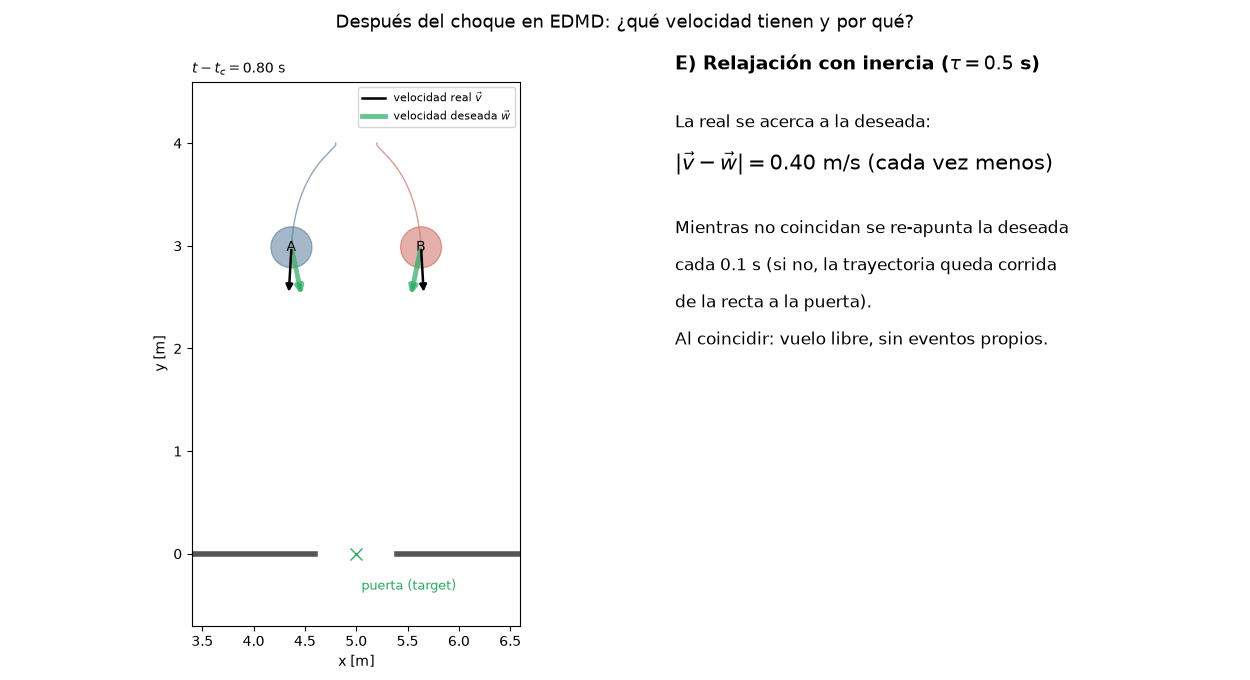
\includegraphics[width=\linewidth,height=0.78\textheight,keepaspectratio]{frame_two.png}}

      \soloentrega{\videolink{dos}}
    \end{column}
    \begin{column}{0.30\textwidth}
      \params{%
        $y = 4\un{m}$, $x = 5\pm(r+1\un{mm})$\\
        puerta en $x = 5\un{m}$\\[4pt]
        Negro: velocidad real.\\
        Verde: velocidad deseada.}
    \end{column}
  \end{columns}
\end{frame}

% =====================================================================
\section{Implementación}
% =====================================================================

% SLIDE impl_uml | V:B | T:20
\begin{frame}{Diagrama de clases del motor}
  \centering
  \begin{tikzpicture}[scale=1.05,
      cls/.style={draw,font=\tiny,align=left,inner sep=2pt,rectangle split,
                  rectangle split parts=2,rectangle split part fill={gray!15,white}},
      comp/.style={-{Diamond[open,length=2.5mm]},thick},
      use/.style={-{Latex[length=2mm]},dashed,gray!70!black}]
    \node[cls] (cfg) at (-4.6,1.6) {\textbf{EvacuationConfig}\nodepart{second}N, L, d, dt, dt$_2$, T, $\alpha$\\sfm: SfmParams};
    \node[cls] (room) at (-4.6,-0.4) {\textbf{Room}\nodepart{second}doorCenter, exitTarget\\walls: WallSet};
    \node[cls] (ag) at (-4.6,-2.2) {\textbf{Agent}\nodepart{second}id, x, v, a, radio\\status, scheme};
    \node[cls] (ed) at (0,1.2) {\textbf{EdmdEngine}\nodepart{second}step(), nextEventTime()\\snapshot(t), release(), admit()};
    \node[cls] (hy) at (0,-1.4) {\textbf{HybridEngine}\nodepart{second}step(), nextTime()\\criterio $\tau_c$, $T$, $\alpha T$};
    \node[cls] (rx) at (4.4,1.6) {\textbf{Relaxation}\nodepart{second}x$_0$, v$_0$, w, t$_0$\\relaxedPosition(t)};
    \node[cls] (fw) at (4.4,-0.2) {\textbf{ForceWorkspace}\nodepart{second}Cell Index Method\\fuerzas SFM (Verlet)};
    \node[cls] (tw) at (4.4,-2.0) {\textbf{TrajectoryWriter}\nodepart{second}writeFrame(t, agentes)\\finish()};
    \draw[comp] (hy) -- node[right,font=\tiny] {edmd\_} (ed);
    \draw[comp] (hy.east) -- ++(0.5,0) |- (fw.west);
    \draw[use] (ed.east) -- (rx.west);
    \draw[use] (hy.south east) -- ++(0.3,-0.5) -| (tw.south);
    \draw[use] (ed.west) -- ++(-0.4,0) |- (cfg.east);
    \draw[use] (hy.west) -- (room.east);
    \draw[use] (hy.south west) -- (ag.east);
    \draw[use] (cfg) -- (room);
  \end{tikzpicture}

  {\scriptsize Rombo: composición. Punteada: usa. TSDMD puro (\texttt{runEvacuation}) usa
  \texttt{ForceWorkspace} directamente.}
\end{frame}

% SLIDE impl_tsdmd | V:B | T:15
\begin{frame}{TSDMD: Velocity Verlet}
  \small
  \begin{align*}
    \vect x(t+dt) &= \vect x(t) + \vect v(t)\,dt + \tfrac12\,\vect a(t)\,dt^2\\
    \vect a(t+dt) &= \vect a\bigl(\vect x(t+dt),\,\vect v(t)+\vect a(t)\,dt\bigr)\\
    \vect v(t+dt) &= \vect v(t) + \tfrac12\bigl[\vect a(t)+\vect a(t+dt)\bigr]\,dt
  \end{align*}
  \begin{itemize}
    \item Fuerza evaluada con la última velocidad disponible (provisoria).
    \item Vecinos con Cell Index Method en cada paso.
    \item Cota de estabilidad: $dt < 0.1\sqrt{m/k}$.
  \end{itemize}
\end{frame}

% SLIDE impl_edmd | V:B | T:25
\begin{frame}{EDMD: cola de eventos}
  \small
  Entre eventos la trayectoria es exacta:
  \[
    \vect x(t) = \vect x_0 + v_d\,\hat{\vect e}\,t
      + (\vect v_0 - v_d\,\hat{\vect e})\,\tau\,(1-e^{-t/\tau})
  \]
  \begin{itemize}
    \item Eventos: contacto (agente, pared, esquina), cruce de celda, puerta, fin del pulso de $0.1\un{s}$.
    \item Cola binaria por tiempo; cada agente tiene un contador de generación (los eventos viejos se descartan).
    \item Tras un choque: se separan las posiciones solapadas más de $1\un{mm}$ (corrección geométrica, no física).
    \item Piso de $5\times10^{-3}\un{s}$ entre choques de un mismo contacto.
  \end{itemize}
\end{frame}

% SLIDE impl_hib_criterio | V:B | T:45
\begin{frame}{Híbrido: criterio de pasaje}
  \centering
  \begin{tikzpicture}[x=1cm,y=1cm]
    \fill[tsdmdc!35] (0,0) rectangle (2.4,1);
    \fill[gray!25]   (2.4,0) rectangle (4.8,1);
    \fill[edmdc!35]  (4.8,0) rectangle (9.5,1);
    \draw[thick] (0,0) rectangle (9.5,1);
    \draw[thick] (2.4,0) -- (2.4,1);
    \draw[thick] (4.8,0) -- (4.8,1);
    \node at (1.2,0.5) {TSDMD};
    \node at (3.6,0.5) {se mantiene};
    \node at (7.15,0.5) {EDMD};
    \node[below] at (0,0) {$0$};
    \node[below] at (2.4,0) {$T$};
    \node[below] at (4.8,0) {$\alpha T$};
    \node[below] at (9.5,0) {$\tau_c$};
  \end{tikzpicture}

  \vspace{8pt}
  \[
    \tau_c(i)=\min\bigl\{t>0:\ |\vect x_i(t)-\vect x_c(t)| = r_i + r_c\bigr\},
    \quad c\in\{\text{agentes, paredes, esquinas}\}
  \]
  \[
    \text{EDMD}\to\text{TSDMD}:\ \tau_c < T
    \qquad
    \text{TSDMD}\to\text{EDMD}:\ \tau_c > \alpha T
  \]
  \vfill
  \params{Retorno además sin contacto y sin colapso (huelgo $<2\un{cm}$ y acercamiento $>5\un{cm/s}$).
          $\alpha = 2$.}
\end{frame}

% SLIDE impl_hib_reloj | V:B | T:55
\begin{frame}{Híbrido: un solo reloj}
  \begin{columns}[c]
    \begin{column}{0.50\textwidth}
      \centering
      \begin{tikzpicture}[x=1cm,y=1cm,
          arr/.style={-{Latex[length=2mm]},thick}]
        \draw[thick] (0,0) -- (5.6,0);
        \foreach \x/\lab in {0.4/{$(k{-}1)dt$}, 2.4/{$k\,dt$}, 4.4/{$(k{+}1)dt$}}{
          \draw[thick] (\x,-0.15) -- (\x,0.15);
          \node[below,font=\scriptsize] at (\x,-0.15) {\lab};
        }
        \draw[arr,tsdmdc] (0.4,0.55) -- node[above,font=\scriptsize] {Verlet} (2.4,0.55);
        \draw[arr,tsdmdc] (2.4,0.55) -- node[above,font=\scriptsize] {Verlet} (4.4,0.55);
        \foreach \x in {0.9,1.5,2.0,3.1,3.4,5.0}
          \fill[edmdc] (\x,-1.25) circle (0.08);
        \node[font=\scriptsize,edmdc,anchor=east] at (-0.1,-1.25) {eventos};
        \node[font=\scriptsize,tsdmdc,anchor=east] at (-0.1,0.55) {TSDMD};
      \end{tikzpicture}
    \end{column}
    \begin{column}{0.46\textwidth}
      \centering
      \begin{tikzpicture}[
          bx/.style={draw,rounded corners,font=\footnotesize,minimum width=5.4cm,minimum height=0.62cm,
                     align=center,inner sep=2pt},
          arr/.style={-{Latex[length=1.8mm]},thick}]
        \node[bx,draw=edmdc]  (a) at (0,0)    {1. eventos EDMD con $t<k\,dt$};
        \node[bx,draw=tsdmdc] (b) at (0,-0.95){2. Verlet de TSDMD hasta $k\,dt$};
        \node[bx]             (c) at (0,-1.9) {3. EDMD avanza a $k\,dt$};
        \node[bx]             (d) at (0,-2.85){4. cruce de puerta y retiro};
        \node[bx,draw=hybc]   (e) at (0,-3.8) {5. EDMD $\to$ TSDMD (y pares mixtos)};
        \node[bx,draw=hybc]   (f) at (0,-4.75){6. TSDMD $\to$ EDMD};
        \foreach \p/\q in {a/b,b/c,c/d,d/e,e/f} \draw[arr] (\p) -- (\q);
      \end{tikzpicture}
    \end{column}
  \end{columns}
  \vfill
  \params{Sin agentes TSDMD no hay límites: el reloj salta de evento en evento.}
\end{frame}

% SLIDE impl_hib_mixto | V:B | T:50
\begin{frame}{Híbrido: par EDMD--TSDMD sin perder contactos}
  \begin{columns}[c]
    \begin{column}{0.46\textwidth}
      \centering
      \begin{tikzpicture}[scale=1.0,
          arr/.style={-{Latex[length=2.2mm]},very thick}]
        \draw[dashed,gray] (2.2,0) circle (1.0);
        \fill[tsdmdc!70] (2.2,0) circle (0.38);
        \fill[edmdc!70] (-1.2,1.0) circle (0.42);
        \node[font=\scriptsize,white] at (2.2,0) {B};
        \node[font=\scriptsize,white] at (-1.2,1.0) {A};
        \draw[arr,edmdc] (-0.8,1.0) -- (0.0,0.75) node[above,font=\scriptsize] {$\vect v_A$};
        \draw[arr,tsdmdc] (2.2,-0.45) -- (2.2,-1.35) node[right,font=\scriptsize] {$\vect v_B$};
        \draw[edmdc,thick,dotted] (0.0,0.75) to[out=-15,in=150] (1.35,0.55);
        \node[font=\scriptsize,gray!60!black] at (3.2,1.25) {$r_A+r_B$};
        \draw[<->,thin] (-1.2,-0.95) -- node[below,font=\scriptsize] {$\tau_c < T$} (1.35,-0.95);
      \end{tikzpicture}
    \end{column}
    \begin{column}{0.52\textwidth}
      \small
      \begin{align*}
        \vect x_A(t) &= \vect x_A + v_d\hat{\vect e}\,t + (\vect v_A - v_d\hat{\vect e})\,\tau\,(1-e^{-t/\tau})\\
        \vect x_B(t) &= \vect x_B + \vect v_B\,t\\
        \tau_c &= \min\{t:\ |\vect x_B(t)-\vect x_A(t)| = r_A+r_B\}
      \end{align*}
      \[
        \tau_c < T \;\Longrightarrow\; A \to \text{TSDMD antes del contacto}
      \]
    \end{column}
  \end{columns}
  \vfill
  \params{El contacto lo resuelve el resorte SFM. El escaneo se repite en cada límite hasta que no haya
          promociones nuevas.}
\end{frame}

% =====================================================================
\section{Simulaciones}
% =====================================================================

% SLIDE sim_sistema | V:C | T:20
\begin{frame}{Sistema simulado}
  \begin{columns}[c]
    \begin{column}{0.44\textwidth}
      \centering
      \begin{tikzpicture}[scale=0.85]
        \draw[thick] (-2,-2) -- (-0.4,-2);
        \draw[thick] (0.4,-2) -- (2,-2);
        \draw[thick] (-2,-2) -- (-2,2) -- (2,2) -- (2,-2);
        \foreach \x/\y in {-1.3/1.2, 0.2/1.5, 1.2/0.9, -0.7/0.2, 0.9/-0.2, -1.4/-0.9, 0.1/-1.0}
          \fill[gray!60] (\x,\y) circle (0.15);
        \draw[<->] (-2,2.3) -- (2,2.3) node[midway,above,font=\scriptsize] {$L$};
        \draw[<->] (-0.4,-2.45) -- (0.4,-2.45) node[midway,below,font=\scriptsize] {$d$};
      \end{tikzpicture}
    \end{column}
    \begin{column}{0.54\textwidth}
      \params{%
        $L = 50\un{m}$, $d = 0.8\un{m}$\\
        $N = 200$ y $N = 500$\\
        $r\in[0.18,\,0.25]\un{m}$, $v_d = 1.5\un{m/s}$\\
        $m = 80\un{kg}$, $\tau = 0.5\un{s}$, $k = 1.2\times10^{5}\un{kg/s^2}$\\
        $dt = 10^{-4}\un{s}$, pulso $0.1\un{s}$\\
        híbrido: $T = 0.5\un{s}$, $\alpha = 2$}

      \vspace{4pt}
      Inicio: agentes al azar sin solape, con velocidad $v_d$ hacia la puerta.
    \end{column}
  \end{columns}
\end{frame}

% SLIDE sim_observables | V:C | T:30
\begin{frame}{Observables}
  \small
  Calculados en post-proceso, desde las trayectorias.
  \begin{align*}
    N_{in}(t) &= \#\{i:\ y_i(t) \geq 0\}, \qquad t_{evac} = \min\{t:\ N_{in}(t)=0\}\\
    \langle t_{evac}\rangle &= \frac1n\sum_{m=1}^{n} t_{evac}^{(m)}, \qquad
      \mathrm{SEM}=\frac{s}{\sqrt n}, \quad s^2=\frac{1}{n-1}\sum_m\bigl(t^{(m)}_{evac}-\langle t_{evac}\rangle\bigr)^2\\
    z &= \frac{\langle t\rangle - \langle t\rangle_{TSDMD}}{\sqrt{\mathrm{SEM}^2+\mathrm{SEM}_{TSDMD}^2}}
  \end{align*}
  \begin{itemize}
    \item Error: SEM, solo sobre corridas completas; $|z|<2$: no se distingue.
    \item $W$: tiempo de ejecución del motor, un hilo.
  \end{itemize}
\end{frame}

% SLIDE sim_rangos | V:C | T:15
\begin{frame}{Qué se varía}
  \begin{itemize}
    \item Esquema: TSDMD, EDMD, híbrido; $\geq 10$ realizaciones completas cada uno.
    \item Umbral del híbrido: $T\in\{0,\,0.1,\,0.25,\,0.5,\,1,\,2,\,3\}\un{s}$.
    \item Cantidad de agentes: $N$ con $L\propto\sqrt{N}$ (densidad fija) y con $L=50\un{m}$.
    \item Las corridas que no evacúan antes de $t_{max}$ no entran al promedio; se informa su cantidad.
  \end{itemize}
\end{frame}

% =====================================================================
\section{Resultados}
% =====================================================================

% SLIDE res_anim | V:C | T:35
\begin{frame}{Esquema: animaciones, sala completa}
  \begin{columns}[T]
    \begin{column}{0.325\textwidth}
      \centering
      \animacion{tsdmd}{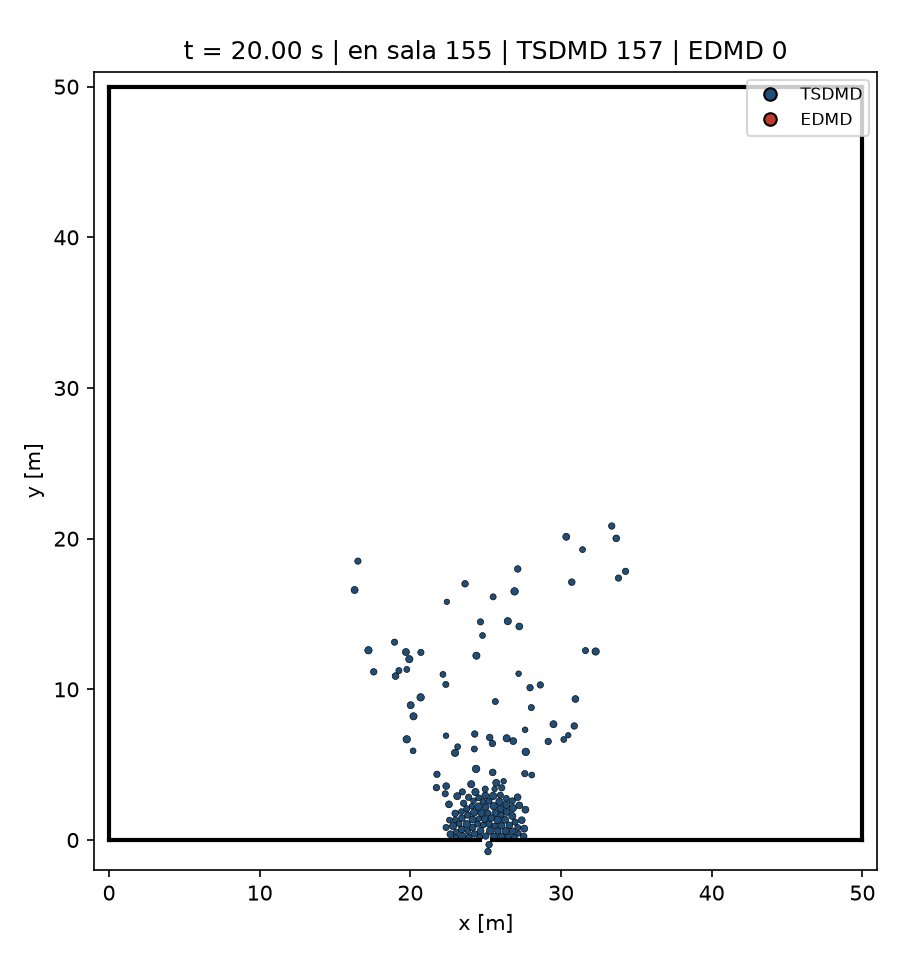
\includegraphics[width=0.74\linewidth]{frame_tsdmd_full.png}}

      {\footnotesize\color{tsdmdc}\textbf{TSDMD}}\\
      \soloentrega{\videolink{tsdmd}}
    \end{column}
    \begin{column}{0.325\textwidth}
      \centering
      \animacion{edmd}{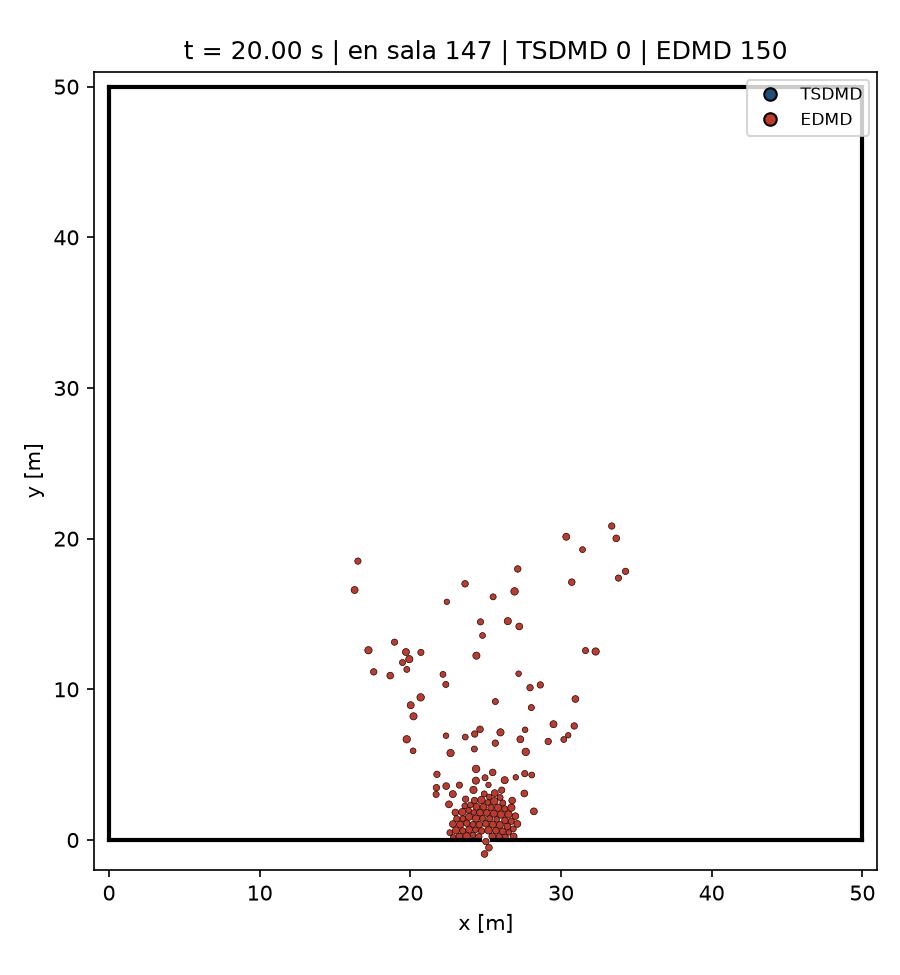
\includegraphics[width=0.74\linewidth]{frame_edmd_full.png}}

      {\footnotesize\color{edmdc}\textbf{EDMD}}\\
      \soloentrega{\videolink{edmd}}
    \end{column}
    \begin{column}{0.325\textwidth}
      \centering
      \animacion{hibrido}{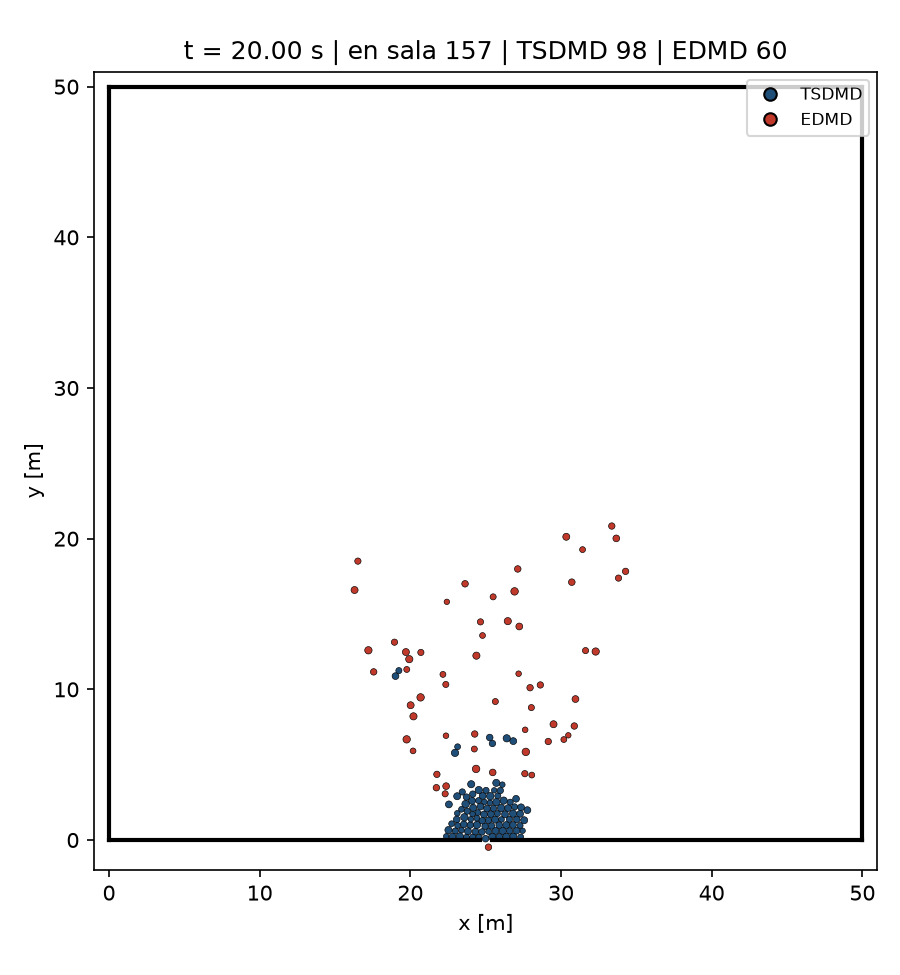
\includegraphics[width=0.74\linewidth]{frame_hybrid_full.png}}

      {\footnotesize\color{hybc}\textbf{Híbrido}}\\
      \soloentrega{\videolink{hibrido}}
    \end{column}
  \end{columns}
  \vfill
  \params{$N = 200$, $L = 50\un{m}$, una realización (semilla 1), $t = 20\un{s}$; $T = 0.5\un{s}$, $\alpha = 2$.}
\end{frame}

% SLIDE res_anim_zoom | V:C | T:25
\begin{frame}{Esquema: animaciones, zoom a la puerta}
  \begin{columns}[T]
    \begin{column}{0.325\textwidth}
      \centering
      \animacion{tsdmd_zoom}{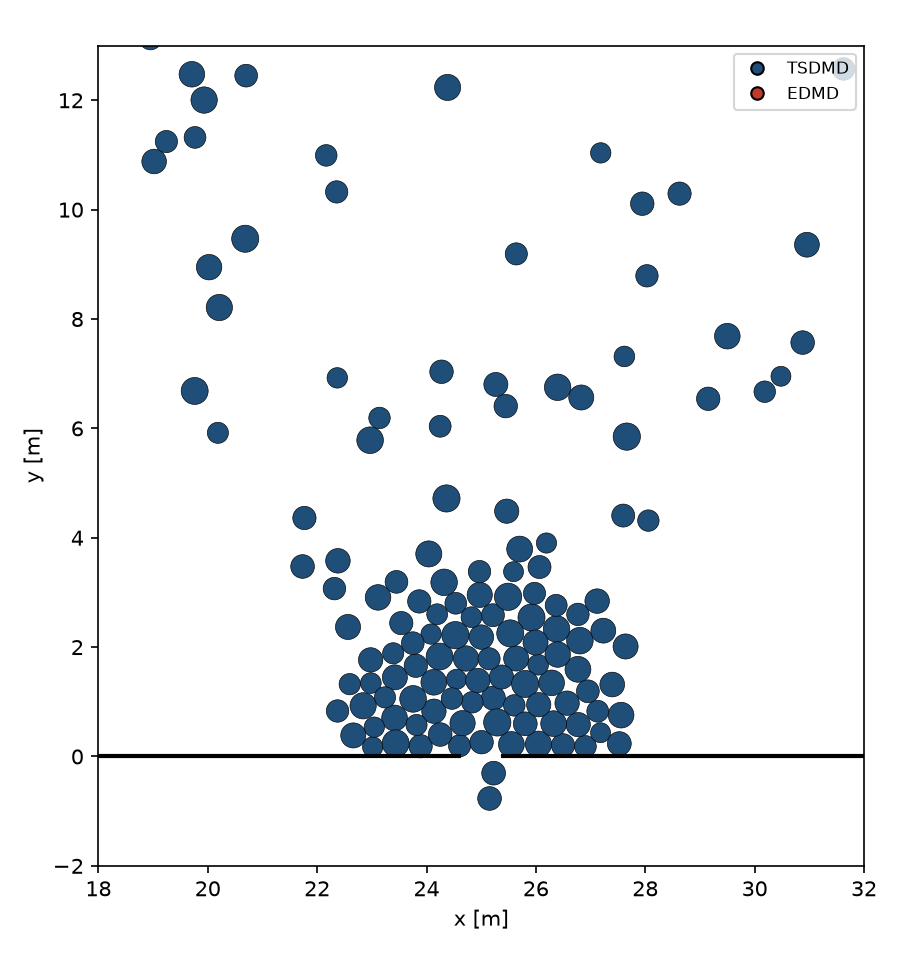
\includegraphics[width=0.8\linewidth]{frame_tsdmd_zoom.png}}

      {\footnotesize\color{tsdmdc}\textbf{TSDMD}}\\
      \soloentrega{\videolink{tsdmd_zoom}}
    \end{column}
    \begin{column}{0.325\textwidth}
      \centering
      \animacion{edmd_zoom}{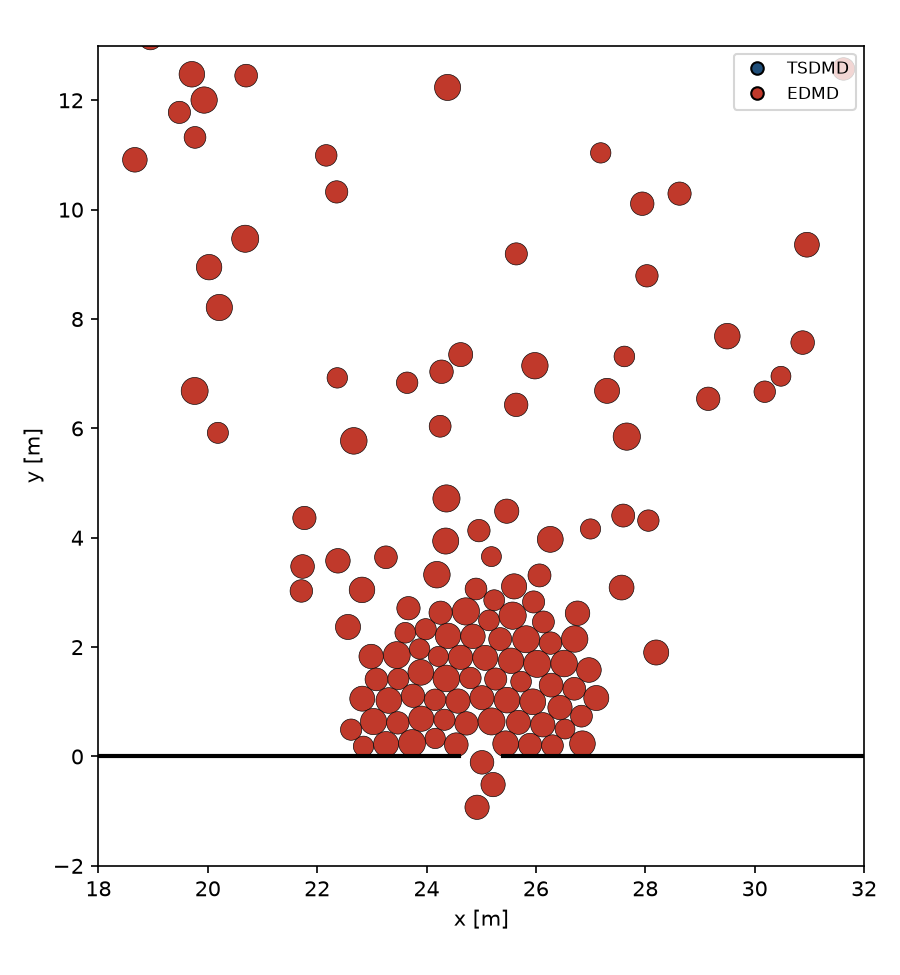
\includegraphics[width=0.8\linewidth]{frame_edmd_zoom.png}}

      {\footnotesize\color{edmdc}\textbf{EDMD}}\\
      \soloentrega{\videolink{edmd_zoom}}
    \end{column}
    \begin{column}{0.325\textwidth}
      \centering
      \animacion{hibrido_zoom}{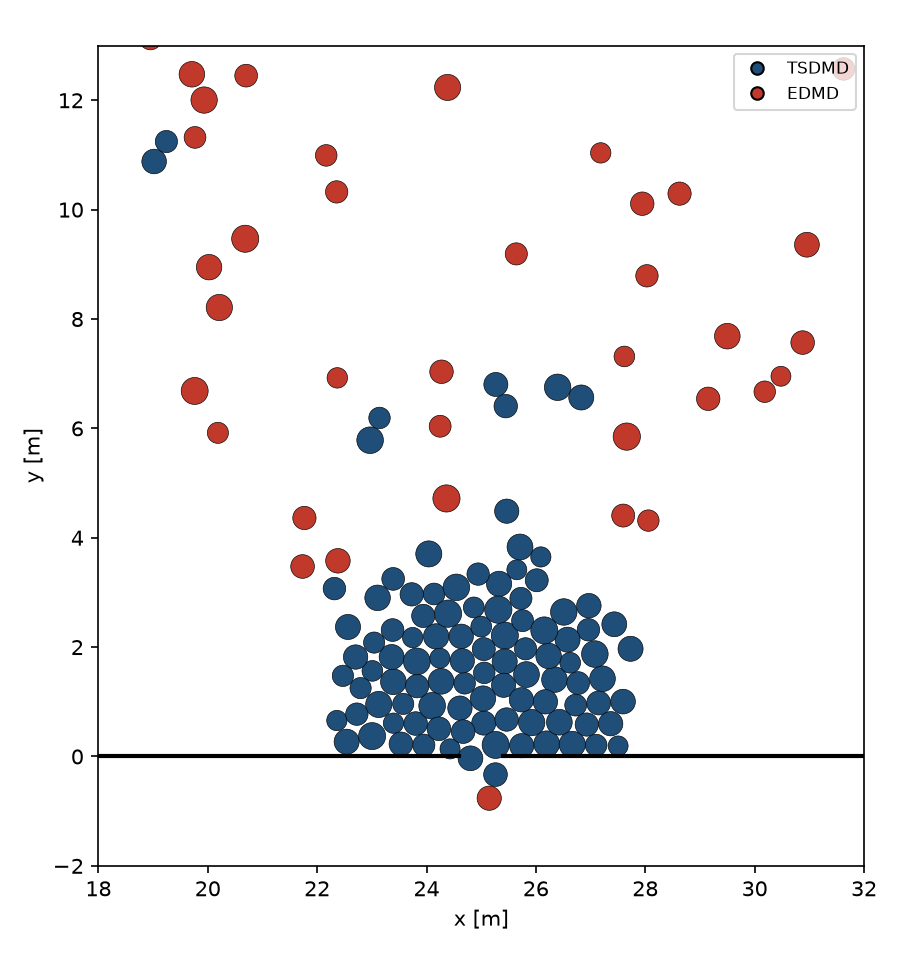
\includegraphics[width=0.8\linewidth]{frame_hybrid_zoom.png}}

      {\footnotesize\color{hybc}\textbf{Híbrido}}\\
      \soloentrega{\videolink{hibrido_zoom}}
    \end{column}
  \end{columns}
  \vfill
  \params{$N = 200$, $L = 50\un{m}$, una realización (semilla 1), $t = 20\un{s}$; $T = 0.5\un{s}$, $\alpha = 2$.}
\end{frame}

% SLIDE res_fraccion | V:A | T:30
\begin{frame}{Híbrido: fracción de agentes en cada esquema}
  \begin{columns}[c]
    \begin{column}{0.64\textwidth}
      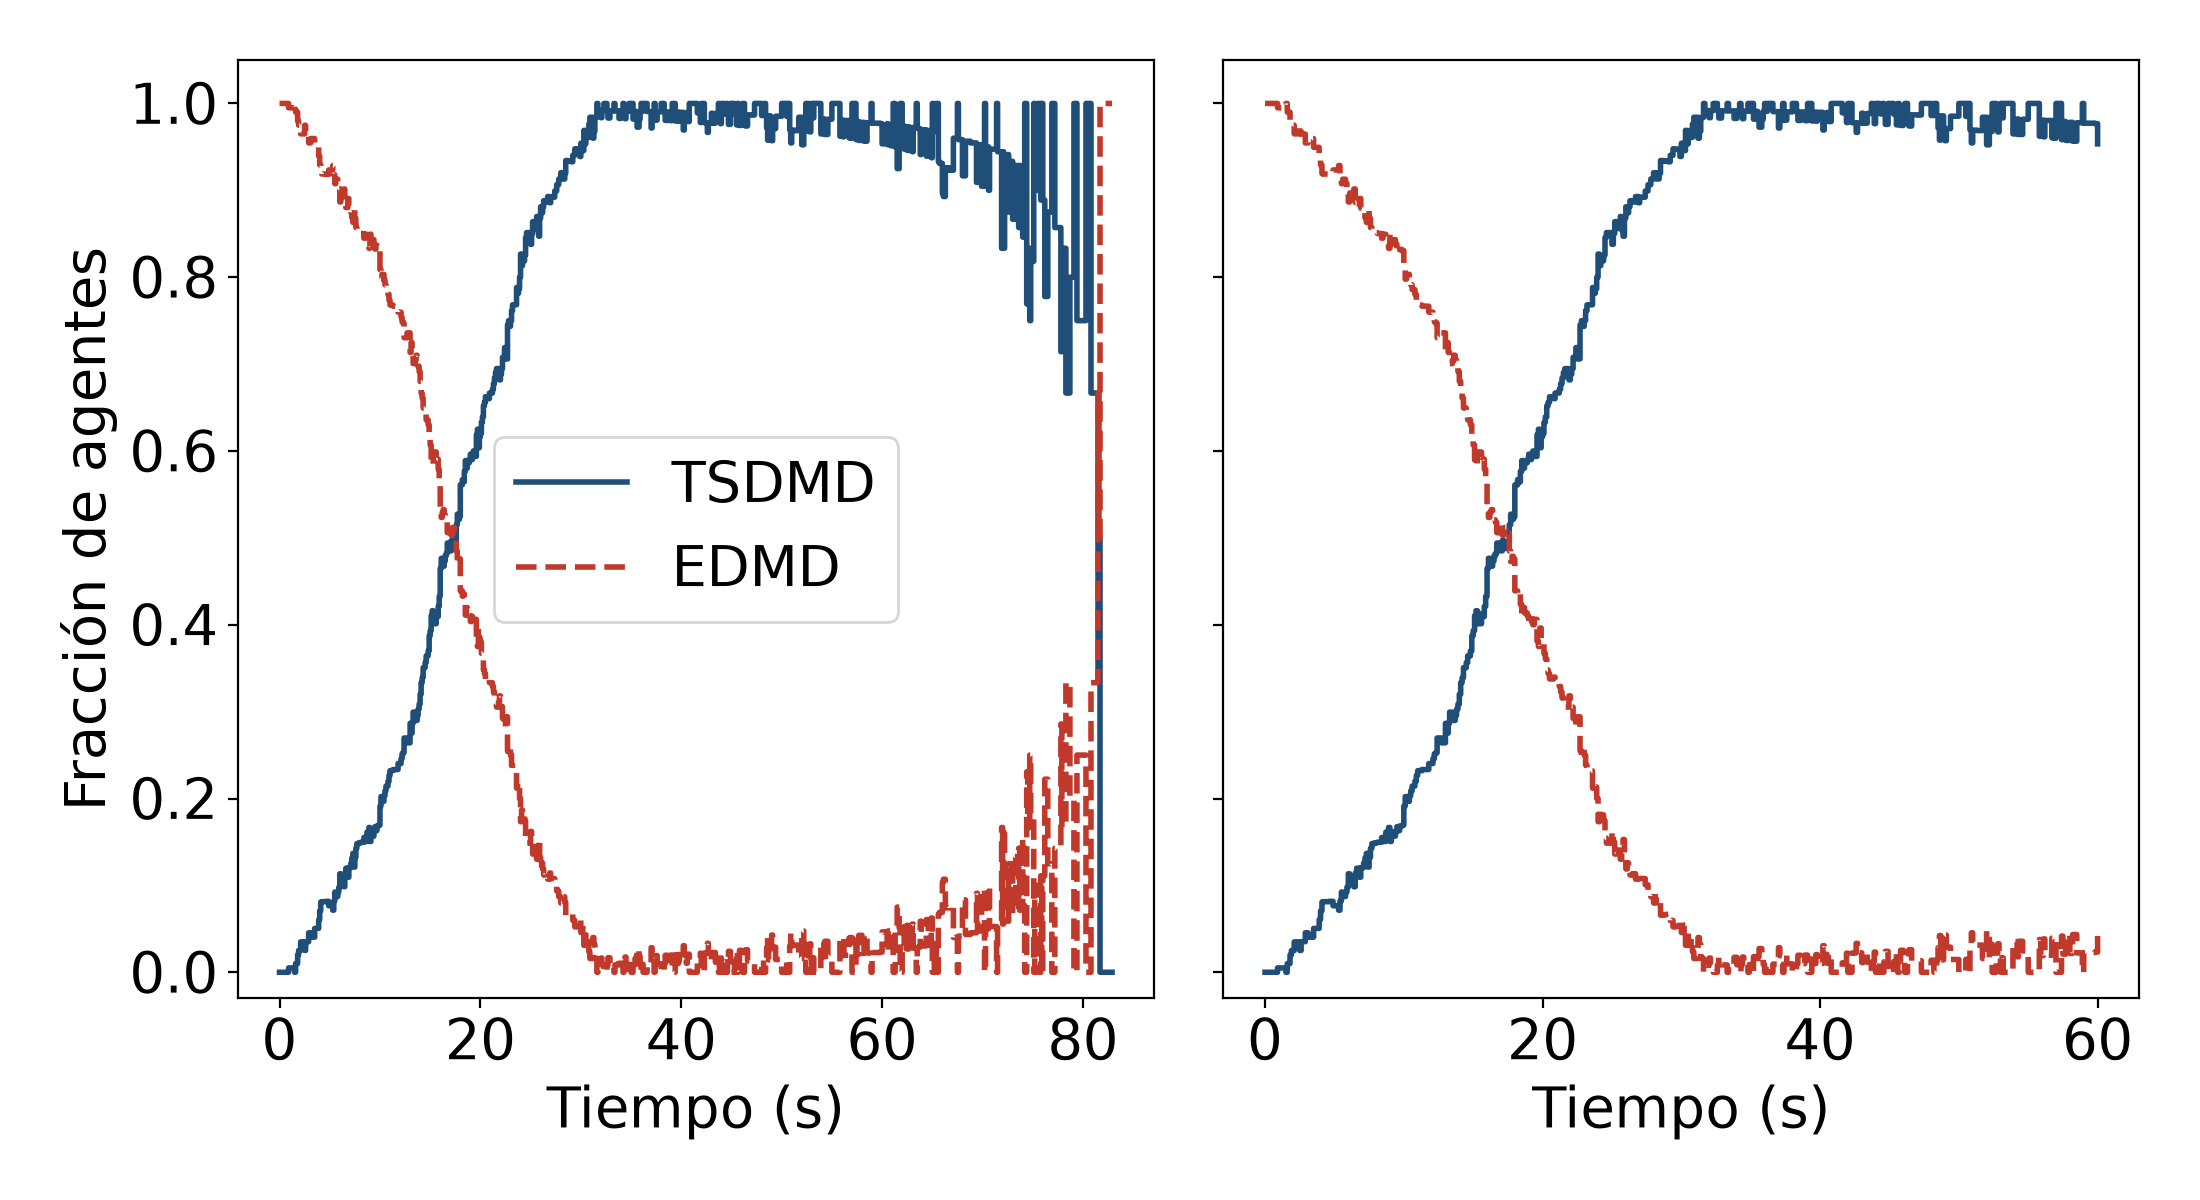
\includegraphics[width=\linewidth,height=0.84\textheight,keepaspectratio]{pres_fraction.png}
    \end{column}
    \begin{column}{0.34\textwidth}
      \params{%
        $N = 200$, $L = 50\un{m}$\\
        $T = 0.5\un{s}$, $\alpha = 2$\\
        Una realización (semilla 1).}
    \end{column}
  \end{columns}
\end{frame}

% SLIDE res_poblacion | V:C | T:25
\begin{frame}{Esquema: población en la sala}
  \begin{columns}[c]
    \begin{column}{0.64\textwidth}
      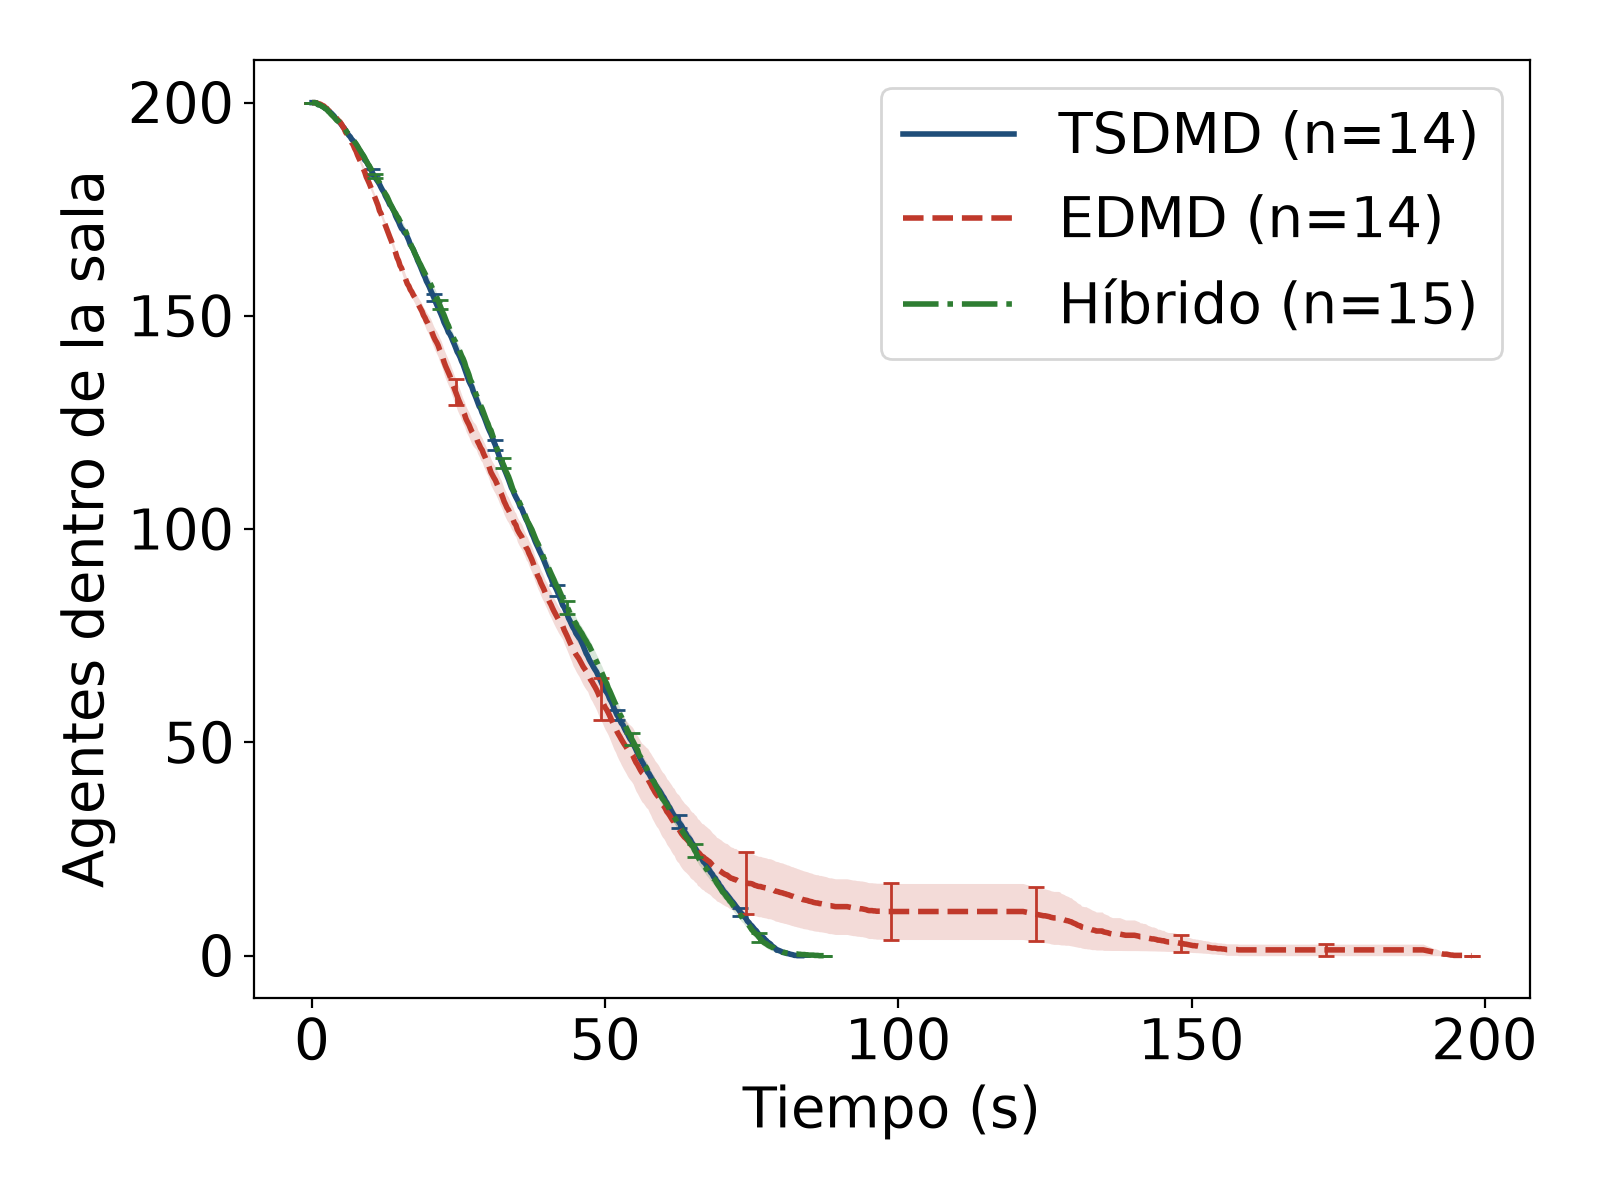
\includegraphics[width=\linewidth,height=0.84\textheight,keepaspectratio]{pres_population.png}
    \end{column}
    \begin{column}{0.34\textwidth}
      \params{%
        $N = 200$, $L = 50\un{m}$\\
        $T = 0.5\un{s}$, $\alpha = 2$\\[4pt]
        Media sobre una grilla común de $t$; solo corridas completas.\\
        Banda: SEM.}
    \end{column}
  \end{columns}
\end{frame}

% SLIDE res_tevac | V:C | T:30
\begin{frame}{Esquema: tiempo de evacuación}
  \begin{columns}[c]
    \begin{column}{0.64\textwidth}
      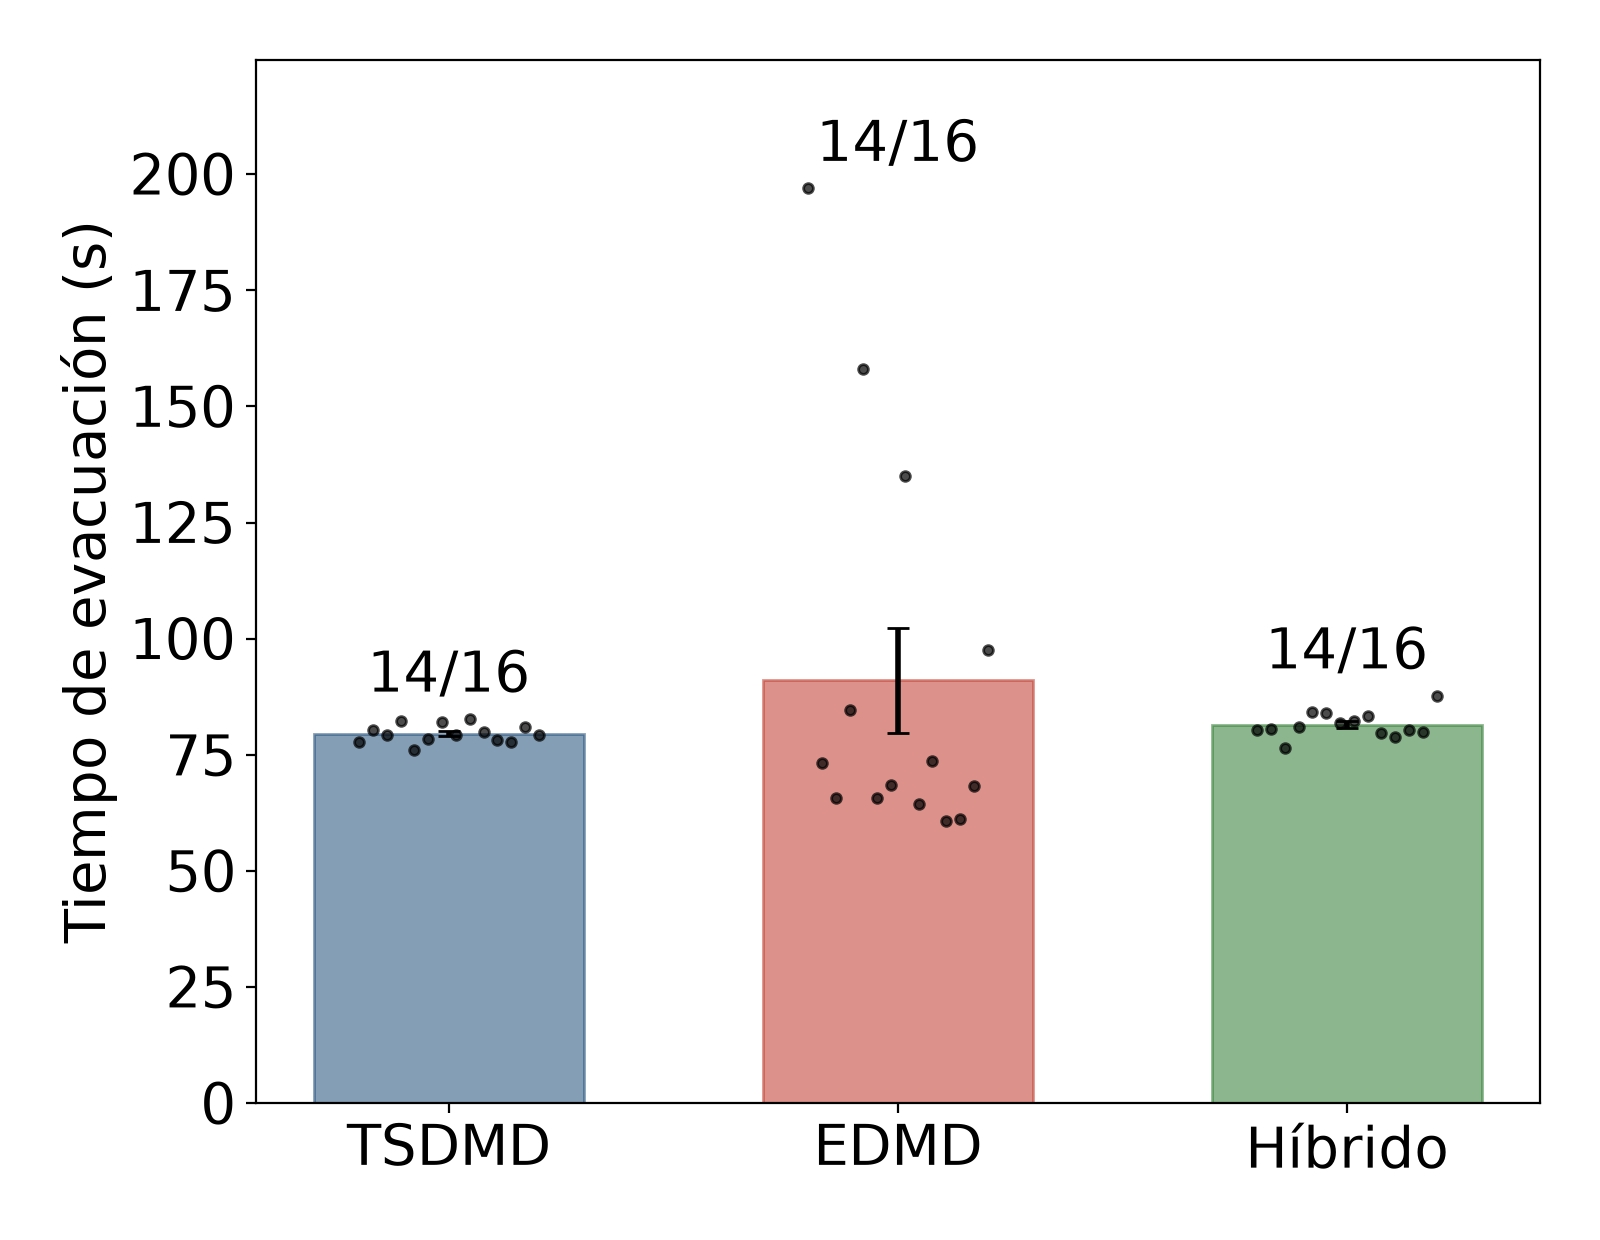
\includegraphics[width=\linewidth,height=0.84\textheight,keepaspectratio]{pres_tevac.png}
    \end{column}
    \begin{column}{0.34\textwidth}
      \params{%
        $N = 200$, $L = 50\un{m}$\\
        Sobre cada barra: corridas completas / intentadas.\\
        Puntos: cada realización.\\[4pt]
        $z$ respecto de TSDMD:\\
        EDMD $1.0$, híbrido $2.1$.}
    \end{column}
  \end{columns}
\end{frame}

% SLIDE res_walltime | V:C | T:20
\begin{frame}{Esquema: tiempo de ejecución}
  \begin{columns}[c]
    \begin{column}{0.64\textwidth}
      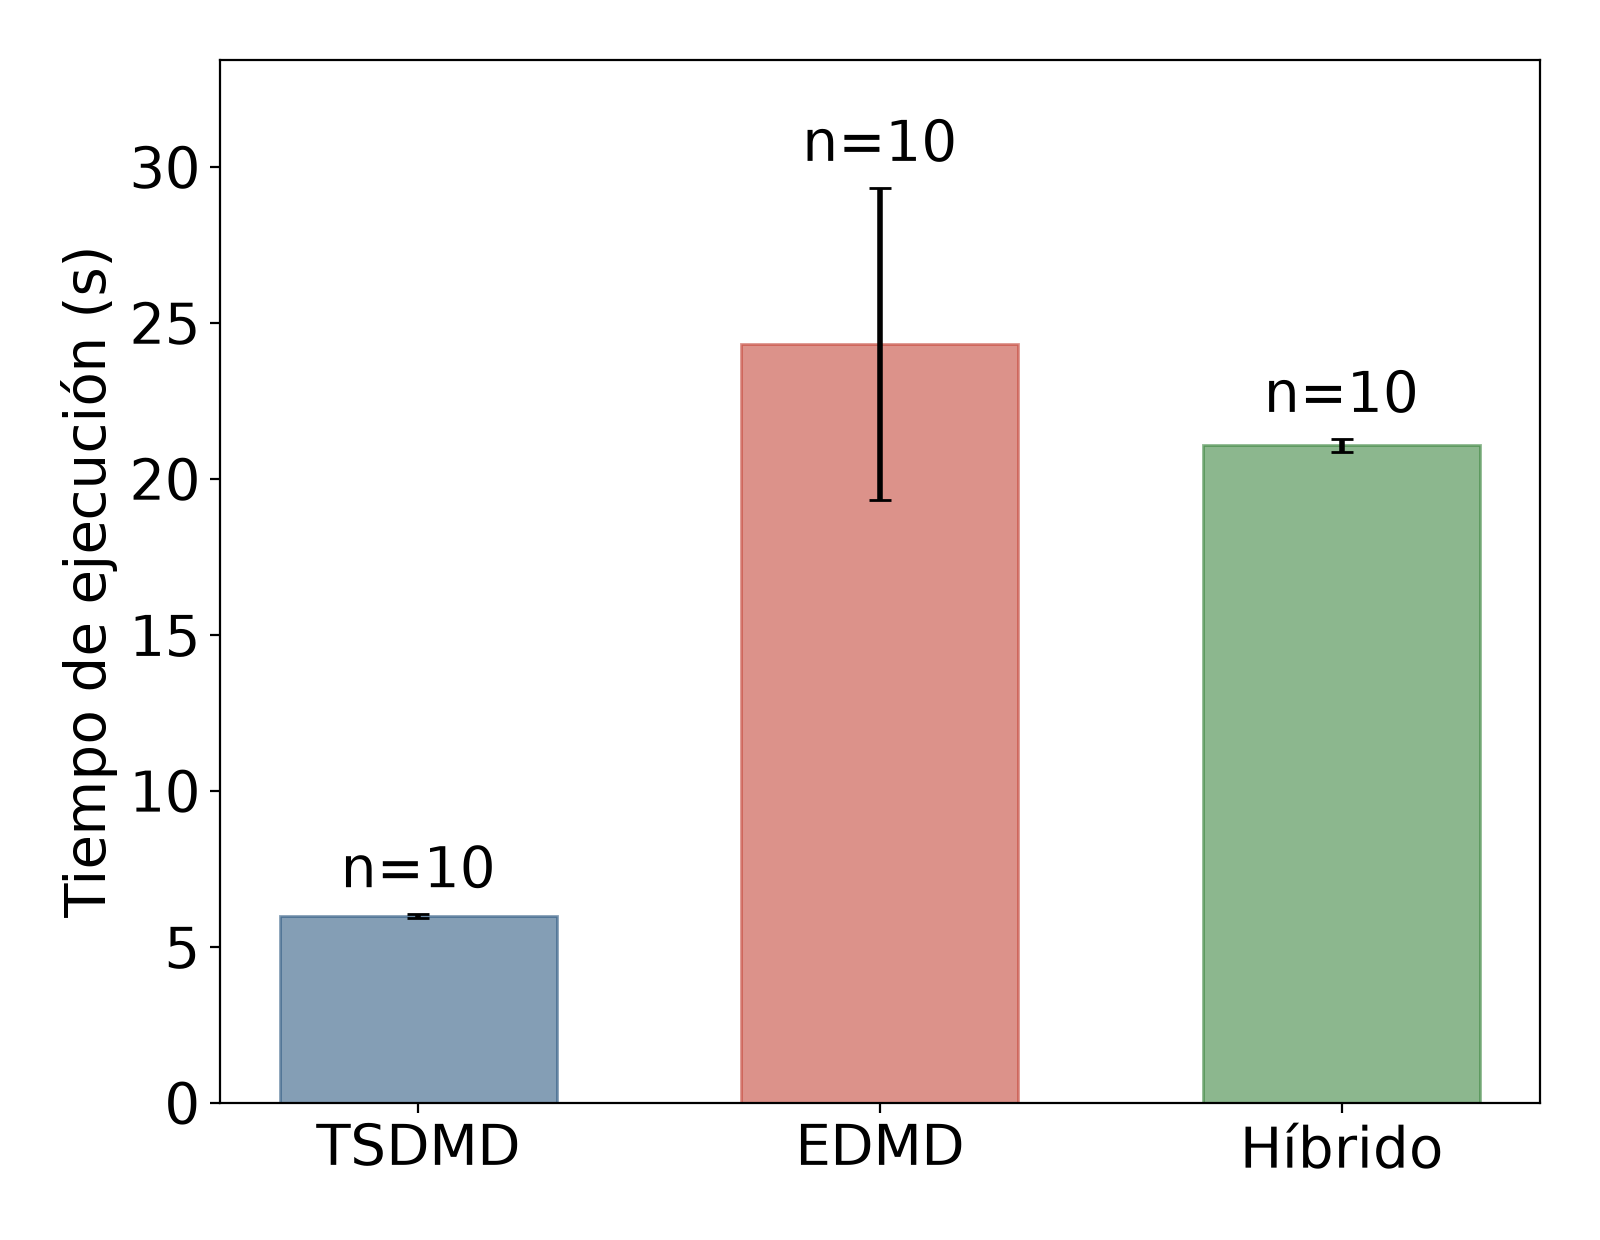
\includegraphics[width=\linewidth,height=0.84\textheight,keepaspectratio]{pres_walltime.png}
    \end{column}
    \begin{column}{0.34\textwidth}
      \params{%
        $N = 200$, $L = 50\un{m}$\\
        Un hilo, misma máquina, corridas en serie.}
    \end{column}
  \end{columns}
\end{frame}

% SLIDE res_sweep | V:A | T:50
\begin{frame}{Umbral $T$ del híbrido}
  \begin{columns}[c]
    \begin{column}{0.50\textwidth}
      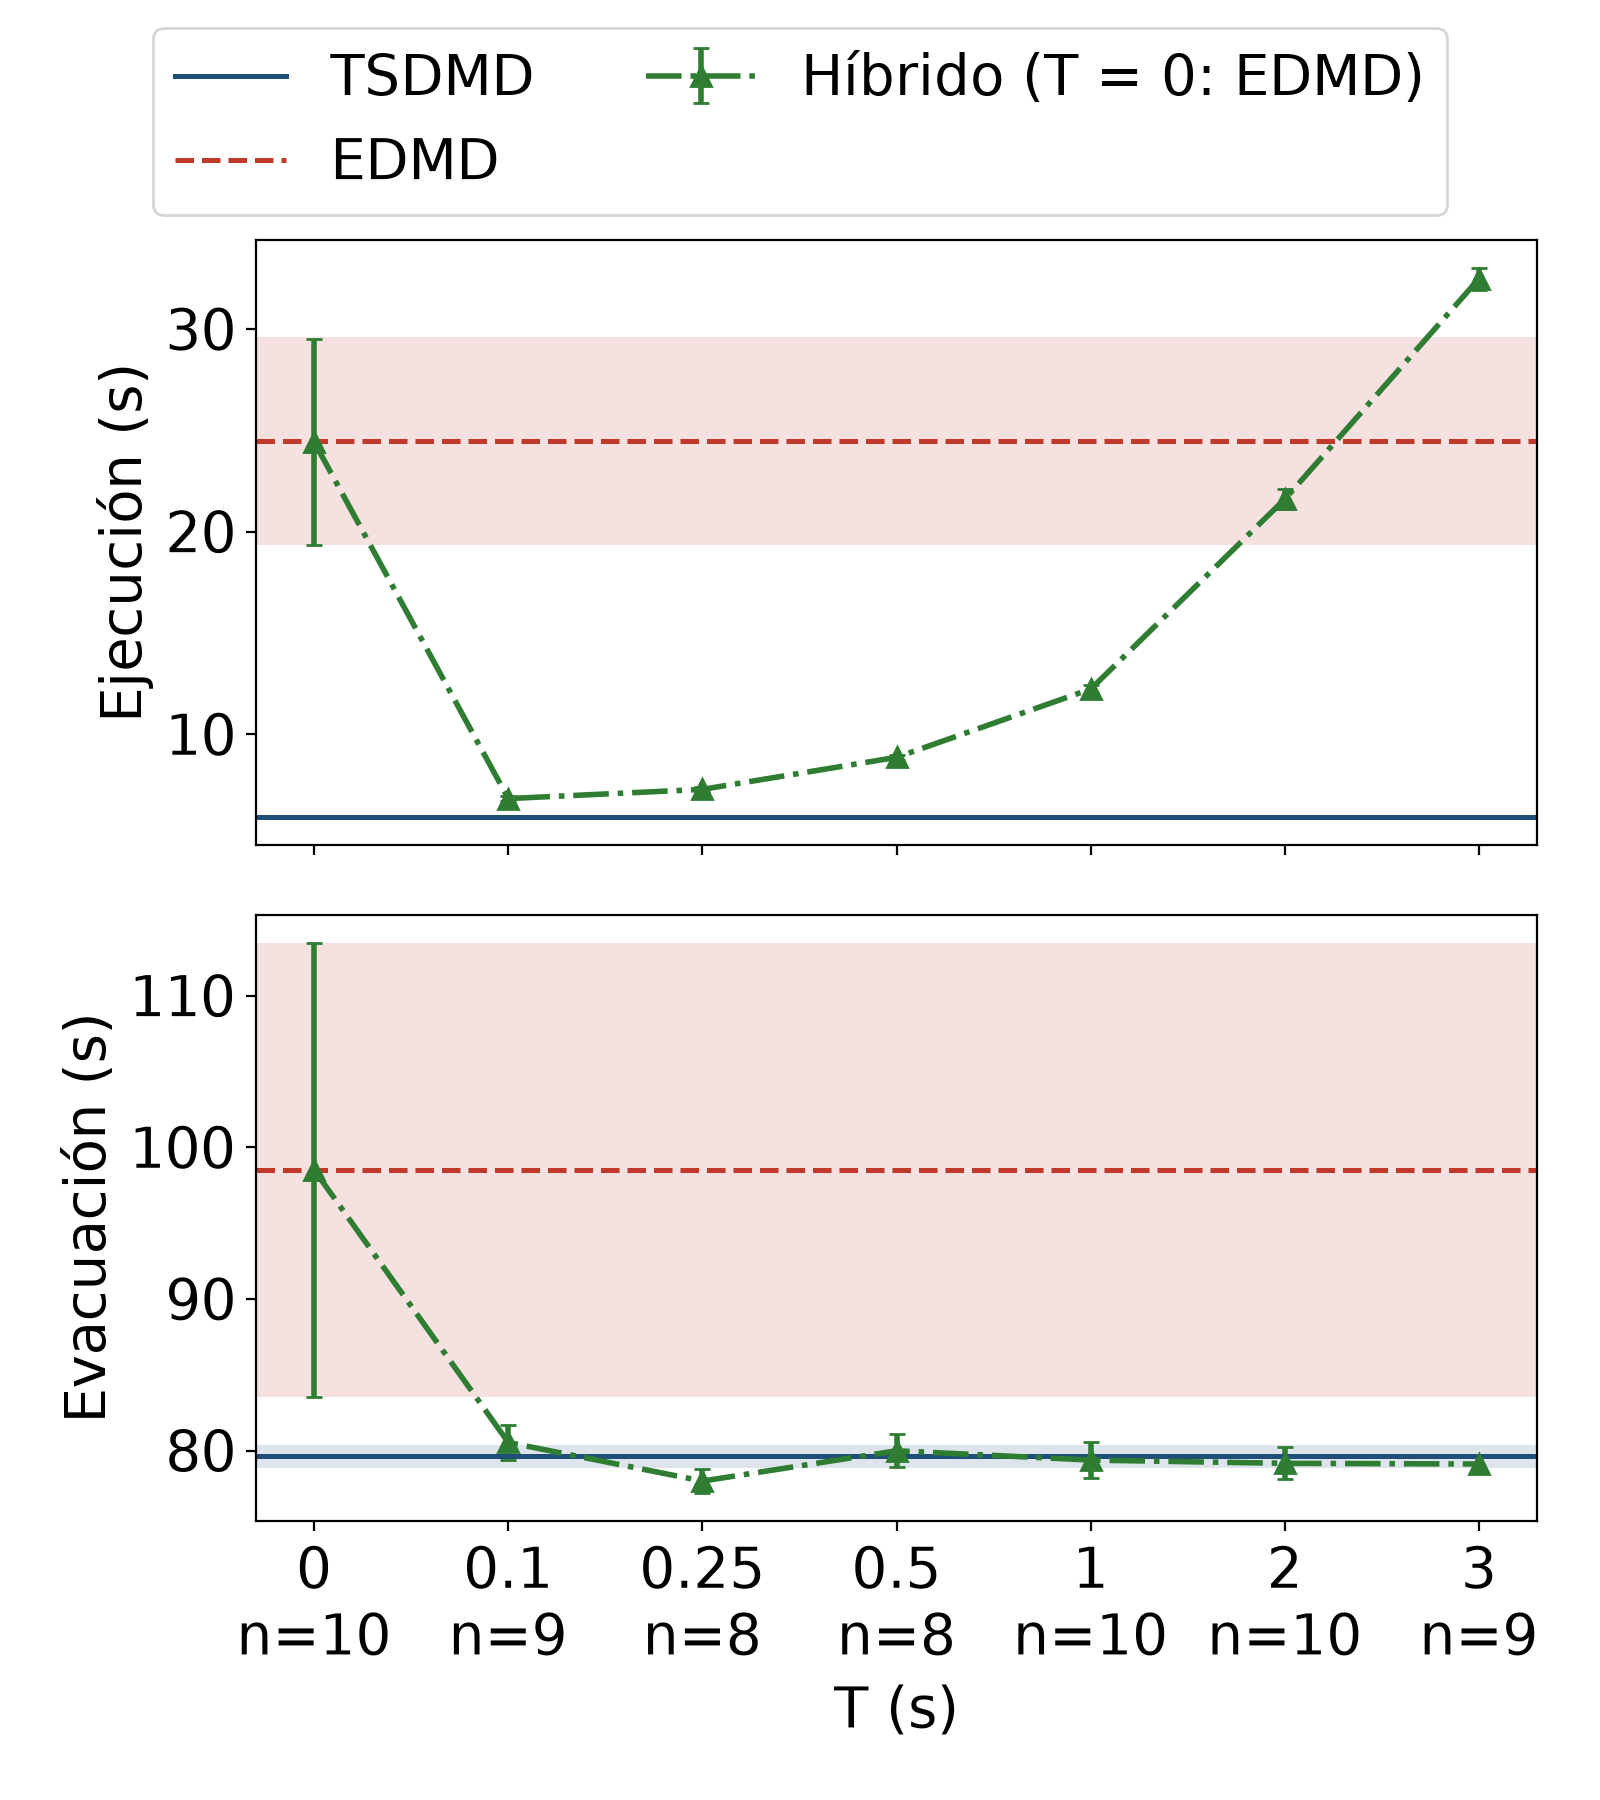
\includegraphics[width=\linewidth,height=0.86\textheight,keepaspectratio]{pres_sweep_T.png}
    \end{column}
    \begin{column}{0.46\textwidth}
      \params{%
        $N = 200$, $L = 50\un{m}$, $\alpha = 2$\\
        10 realizaciones por punto; $n$ bajo cada $T$: las completas.\\[4pt]
        $T = 0$: reproduce el EDMD puro.\\
        Franjas: SEM de TSDMD y EDMD.}
    \end{column}
  \end{columns}
\end{frame}

% SLIDE res_escala_a | V:A | T:25
\begin{frame}{Escalado con $N$: densidad fija}
  \begin{columns}[c]
    \begin{column}{0.64\textwidth}
      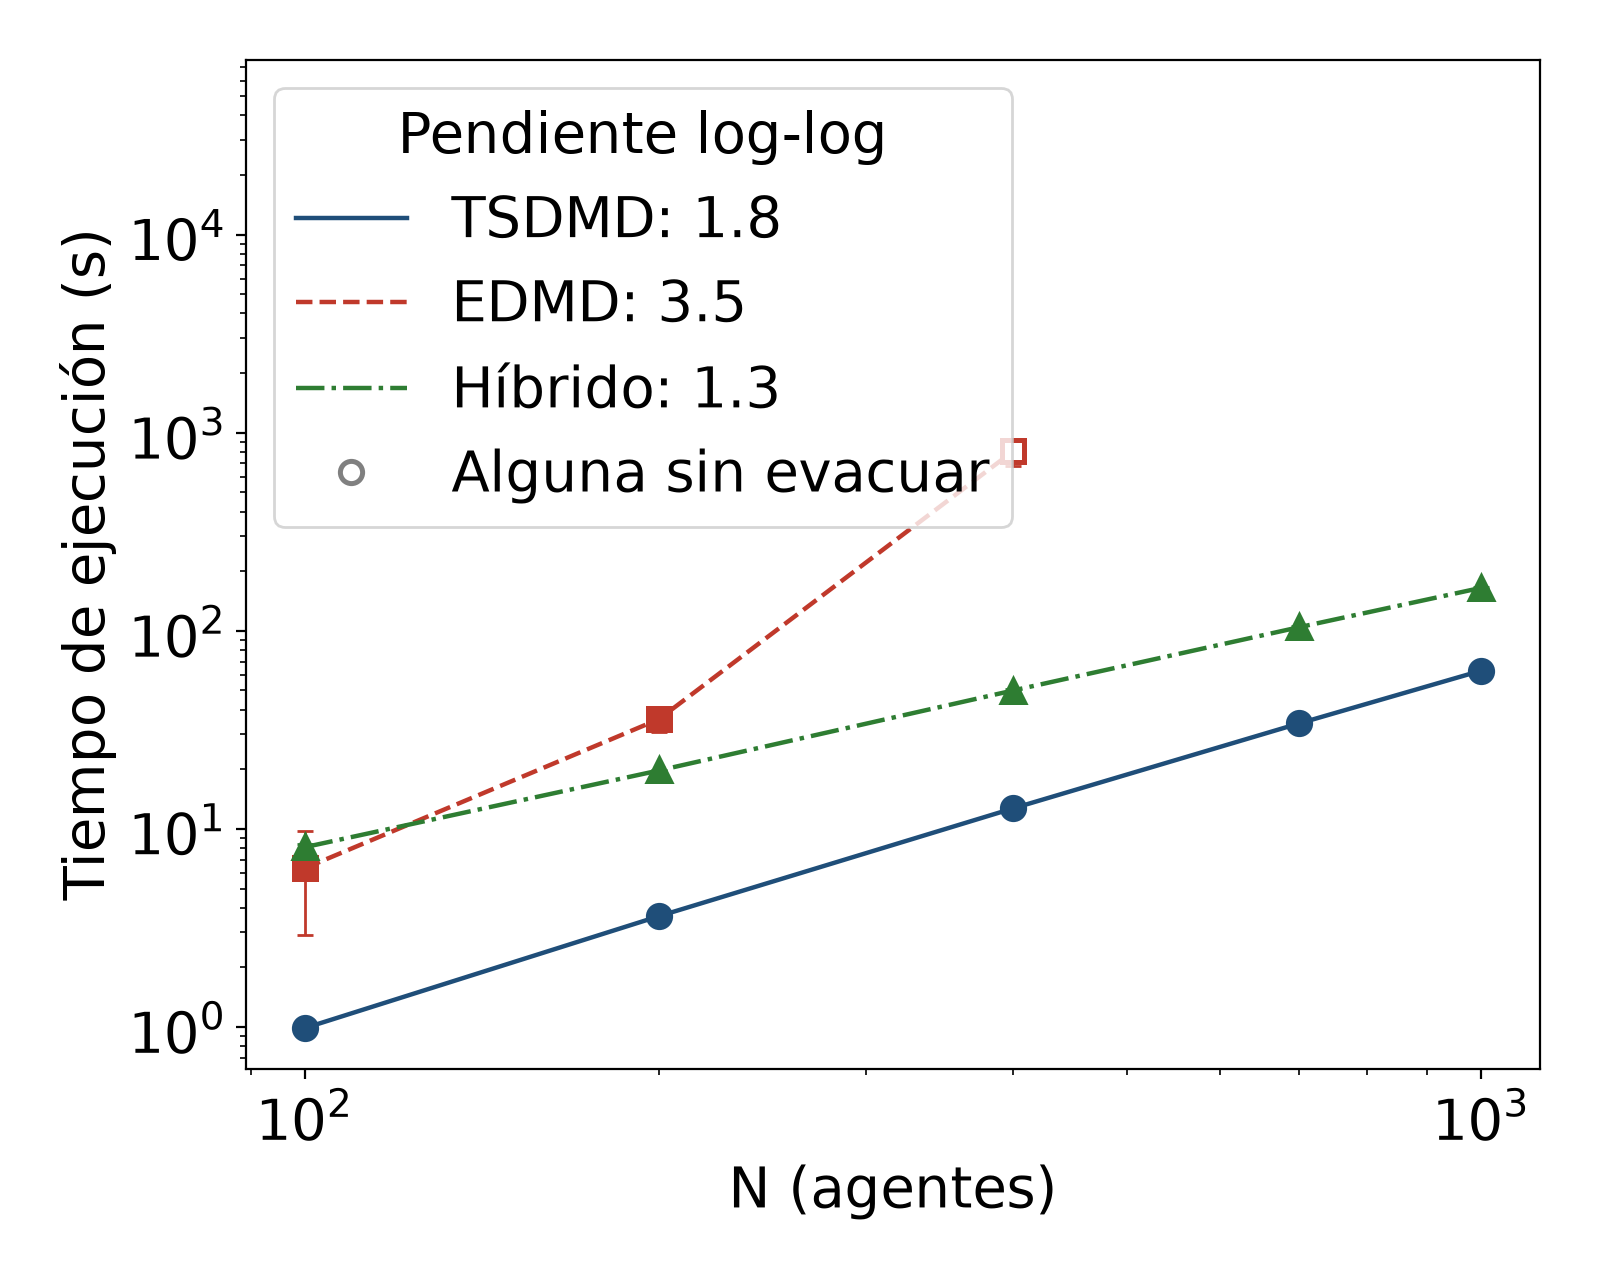
\includegraphics[width=\linewidth,height=0.84\textheight,keepaspectratio]{pres_scale_a.png}
    \end{column}
    \begin{column}{0.34\textwidth}
      \params{%
        $L = 50\sqrt{N/500}\un{m}$\\
        \textbf{3 realizaciones por punto} (menos que las 10 del resto): el error es poco confiable; vale la tendencia, no el valor.\\
        Hueco: alguna corrida no evacuó antes de $t_{max}$.\\
        Pendiente: ajuste lineal de $\log W$ contra $\log N$ sobre todos los puntos.}
    \end{column}
  \end{columns}
\end{frame}

% SLIDE res_escala_b | V:A | T:20
\begin{frame}{Escalado con $N$: $L$ fija}
  \begin{columns}[c]
    \begin{column}{0.64\textwidth}
      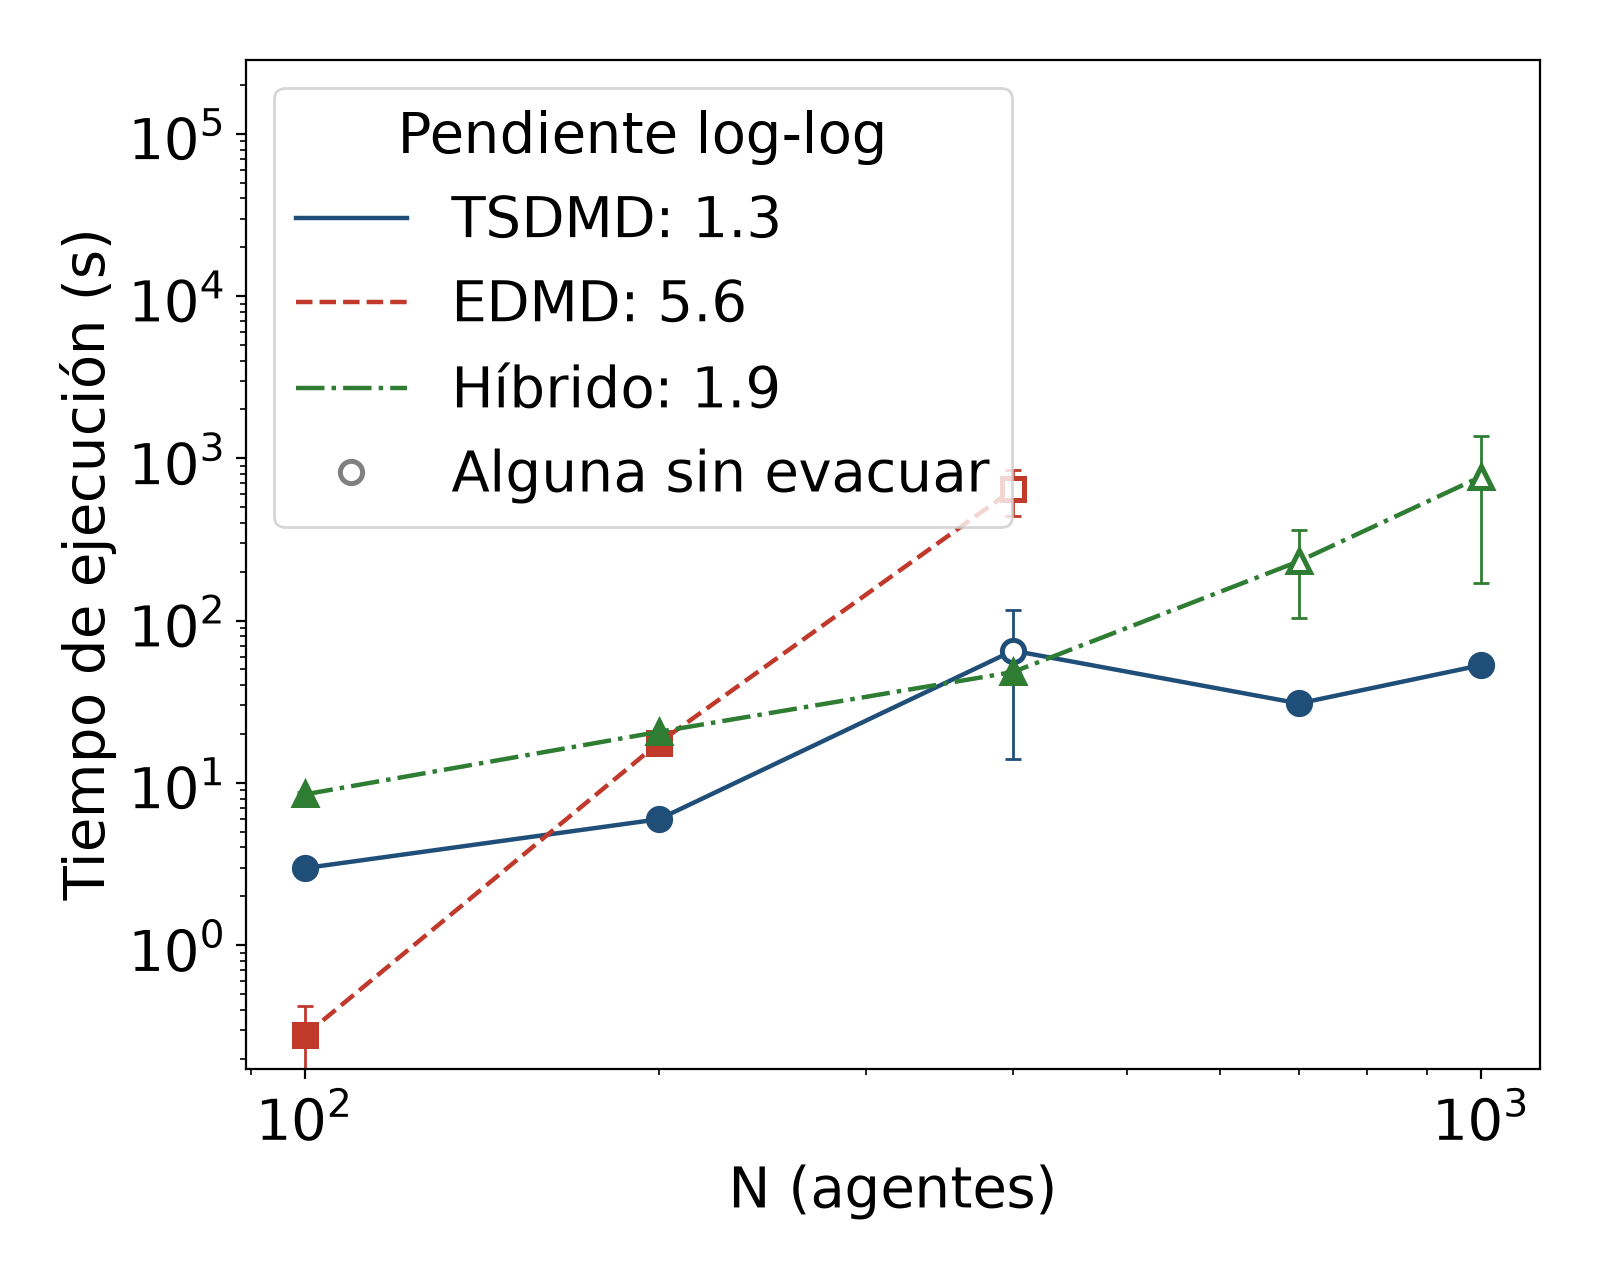
\includegraphics[width=\linewidth,height=0.84\textheight,keepaspectratio]{pres_scale_b.png}
    \end{column}
    \begin{column}{0.34\textwidth}
      \params{%
        $L = 50\un{m}$ (la densidad crece con $N$).\\
        \textbf{3 realizaciones por punto} (menos que las 10 del resto): el error es poco confiable; vale la tendencia, no el valor.}
    \end{column}
  \end{columns}
\end{frame}

% =====================================================================
\section{Conclusiones}
% =====================================================================

% SLIDE concl | V:B | T:30
\begin{frame}{Conclusiones}
  % Sin valores numericos (Guia 2.5). Cada afirmacion sale de z (|z|<2: no se distingue) o de las tasas
  % de exito; los z estan en res_tevac y en res_sweep.
  \begin{enumerate}
    \small
    \item El EDMD no se distingue del TSDMD en el tiempo medio de evacuación; sí en la dispersión, mucho mayor.
    \item El híbrido y el TSDMD tienen tiempos de evacuación muy cercanos: no se distinguen con 10 realizaciones y con 16 quedan al borde del criterio.
    \item Los tres esquemas dejan corridas sin completar, en proporciones parecidas: los atascos no son propios del EDMD.
    \item El costo de ejecución del híbrido no baja del TSDMD para ningún $T$ evaluado, y es menor que el del EDMD solo para $T$ chico.
    \item $T = 0$ reproduce el EDMD. Con $T$ grande el tiempo de evacuación no se distingue del TSDMD, pero el costo es mayor.
    \item El costo del EDMD crece con $N$ mucho más rápido que el de los otros dos; solo se midió hasta $N = 400$ y con 3 realizaciones: es una tendencia, no un exponente.
  \end{enumerate}
\end{frame}

% SLIDE gracias | V:A | T:3
\begin{frame}[plain]
  \vfill
  \centering
  {\Huge \textbf{Muchas gracias}}
  \vfill
\end{frame}

% =====================================================================
%  Apendice (T:0)
% =====================================================================
\appendix

% SLIDE apx_kappa | V:A | T:0
\begin{frame}{Apéndice: con rozamiento tangencial}
  \footnotesize
  \params{TSDMD, $N = 200$, $L = 50\un{m}$, 10 semillas iguales en ambas filas, $t_{max} = 3000\un{s}$.}
  \begin{center}
    \begin{tabular}{rcc}
      \toprule
      $\kappa\;[\mathrm{kg/(m\,s)}]$ & Evacuaciones completas & $t_{evac}$ (solo completas) \\ \midrule
      $0$ (usado en el trabajo)  & 9/10 & $79.6 \pm 0.8\un{s}$ \\
      $2.4\times10^{5}$ (Helbing) & 4/10 & $364 \pm 13\un{s}$ \\
      \bottomrule
    \end{tabular}
  \end{center}
  \begin{itemize}
    \item Con rozamiento, 6 de 10 corridas terminan antes de $t_{max}$ con entre $14$ y $136$ agentes en sala.
    \item Sin rozamiento, la corrida que no completa (semilla 7) queda con $12$.
    \item El $t_{evac}$ con rozamiento promedia solo 4 corridas: no es comparable con el de $\kappa = 0$.
    \item Por eso todos los esquemas corren con $\kappa = 0$.
  \end{itemize}
\end{frame}

% SLIDE apx_dtc | V:A | T:0
\begin{frame}{Apéndice: duración del pulso}
  \footnotesize
  \params{EDMD, $N = 200$, $L = 50\un{m}$, 10 semillas iguales en las tres filas, $t_{max} = 600\un{s}$.}
  \begin{center}
    \begin{tabular}{rcc}
      \toprule
      $\Delta t_c$ & Evacuaciones completas & $t_{evac}$ (solo completas) \\ \midrule
      $0.05\un{s}$ & 9/10  & $130 \pm 40\un{s}$ \\
      $0.1\un{s}$  & 10/10 & $99 \pm 15\un{s}$ \\
      $0.2\un{s}$  & 0/10  & --- \\
      \bottomrule
    \end{tabular}
  \end{center}
  \begin{itemize}
    \item $t_{evac}$ depende de $\Delta t_c$: es un parámetro del modelo, no un paso numérico.
    \item $0.2\un{s}$: en 9 de 10 corridas queda 1 agente sin cruzar y en la otra, 158.
          Con la semilla 1 el agente rebota entre las dos esquinas de la puerta cada $\approx 0.8\un{s}$.
    \item Hipótesis, sin probar: el pulso ($1.5\un{m/s}\times0.2\un{s}=0.3\un{m}$) es casi el hueco útil
          ($2(0.4-0.25)=0.3\un{m}$) y lo lleva a la esquina opuesta.
    \item $0.05\un{s}$: en 1 de 10 el EDMD se frena con 79 agentes en sala (cascada de choques).
    \item Elegimos $0.1\un{s}$: es el único valor sin fallas en estas 10 semillas.
  \end{itemize}
\end{frame}

% SLIDE apx_dt | V:A | T:0
\begin{frame}{Apéndice: convergencia en $dt$ y reproducibilidad}
  \footnotesize
  \params{$N = 200$, $L = 50\un{m}$; TSDMD 10 semillas, híbrido ($T = 0.5\un{s}$) 5 semillas.}
  \begin{center}
    \begin{tabular}{lcc}
      \toprule
      & $dt = 10^{-4}\un{s}$ & $dt = 5\times10^{-5}\un{s}$ \\ \midrule
      TSDMD   & $79.6 \pm 0.8\un{s}$ & $81.6 \pm 1.6\un{s}$ \\
      Híbrido & $80.4 \pm 1.2\un{s}$ & $81.0 \pm 0.7\un{s}$ \\
      \bottomrule
    \end{tabular}
  \end{center}
  \begin{itemize}
    \item Con $dt/2$ no se distingue el $t_{evac}$ (diferencias dentro del error); el costo se duplica.
    \item Una de las 10 semillas del TSDMD no completa con ninguno de los dos $dt$.
    \item Reproducibilidad del EDMD: la misma semilla da trayectorias distintas con otro $t_{max}$
          (separación visible antes de $t = 10\un{s}$), pero idénticas con otro intervalo de salida.
    \item Causa probable (no aislada): la bisección del cruce de plano usa $t_{max}-t$ como intervalo;
          cambia la raíz en $\sim10^{-13}\un{s}$ y el caos de los choques lo amplifica.
    \item Todos los estudios usan el mismo $t_{max}$ por esquema; con $t_{max}$ fijo, las corridas se repiten dígito a dígito.
  \end{itemize}
\end{frame}

% SLIDE apx_ia | V:A | T:0
\begin{frame}{Apéndice: uso de IA}
  \begin{itemize}
    \item Herramienta: Claude Code. Escribió código del motor, \emph{scripts}, figuras y esta presentación.
    \item En la primera versión el agente tomó decisiones de modelo que no habíamos pedido ni entendíamos.
    \item La clase de consultas lo dejó en evidencia: no podíamos explicar la regla de colisión del EDMD.
    \item Rehicimos el EDMD y el híbrido: las reglas las definimos en papel y la IA solo las implementa.
    \item Las siguientes diapositivas listan las libertades que corregimos; la más grande, el EDMD.
  \end{itemize}
\end{frame}

% SLIDE apx_ia_edmd | V:A | T:0
\begin{frame}{Libertades de la IA en el EDMD: antes y después de la consulta}
  \footnotesize
  \begin{tabularx}{\textwidth}{@{}p{0.17\textwidth}XX@{}}
    & \textbf{Lo que hizo la IA} & \textbf{Cómo quedó} \\ \midrule
    Colisión
      & Choque elástico con impulso y coeficiente de restitución $e<1$, copiado del TP3; nadie lo había pedido.
      & Regla propia: $\hat e_{tmp}=\mathrm{norm}(\hat n_{alejar}+\hat e_{target})$ y $|\vect v|=v_d$ en el choque (como el CPM). \\
    Recuperación
      & Evento de $0.1\,\mathrm{s}$ \emph{siempre}, aun con la velocidad ya igual a la deseada: en la práctica un \emph{time step}.
      & Pulso de $0.1\,\mathrm{s}$, relajación exacta con inercia y re-apuntado hasta $|\vect v-v_d\hat e|\le\varepsilon$; después vuelo libre sin eventos. \\
    Choque en plena relajación
      & No estaba definido.
      & Se reaplica la regla con la velocidad actual y el pulso reinicia. \\
    Solapes
      & Parche \texttt{--overlap-cap} que además anulaba velocidades.
      & Se corrigen solo posiciones, y lo decimos: es geométrico, no físico. \\
    Verificación
      & Ninguna con casos simples.
      & Test y animación con $2$ partículas que muestra $\hat e$ deseada y real. \\
  \end{tabularx}
\end{frame}

% SLIDE apx_ia_otras | V:A | T:0
\begin{frame}{Otras libertades que corregimos}
  \footnotesize
  \begin{itemize}
    \item \textbf{Rozamiento tangencial:} la IA lo dejó activo en los tres esquemas y se atascaba. Ahora no está; la comparación va en un apéndice.
    \item \textbf{Agente que no cruza la puerta (EDMD):} apuntaba justo a $y=0$ y se acercaba sin cruzar (Zeno). Apunta $1\,\mathrm{cm}$ por debajo; re-corrimos los estudios.
    \item \textbf{Híbrido:} promovía a TSDMD el vecino recién en el límite siguiente; ahora se repite hasta punto fijo.
    \item \textbf{Comparación justa:} tmax distinto por esquema; ahora el mismo, con tope de \emph{wall-clock}.
    \item \textbf{Estadística:} afirmaba mecanismos como resultado y escribía ``es igual''; ahora ``no se distingue'', con tasa de éxito y 1 cifra significativa.
  \end{itemize}
\end{frame}

\end{document}
